\documentclass[czech,bachelor]{../../shared/diploma}

% Sablonove baliky
\usepackage[autostyle=true,czech=quotes]{csquotes} % korektni sazba uvozovek, podpora pro balik biblatex
\usepackage[backend=biber, style=iso-numeric, alldates=iso]{biblatex} % bibliografie
\usepackage{dcolumn} % sloupce tabulky s ciselnymi hodnotami
\usepackage{subfig} % makra pro "podobrazky" a "podtabulky"

% Moje baliky
\usepackage{float} % lepsi umistovani obrazku (H)
\usepackage{glossaries} % balik pro praci s odbornymi pojmy
\usepackage{hyperref} % vkladani hypertextovych odkazu
\usepackage{xurl} % zalomeni dlouhych URL
\usepackage{tablefootnote} % poznámky pod tabulkou

% Pozadovane vstupy pro generovani titulnich stran.
\ThesisAuthor{Barbora Kovalská}
\ThesisSupervisor{Ing. Radoslav Fasuga, Ph.D.}

\CzechThesisTitle{Tvorba herního modelu výpravné evoluční hry}
\EnglishThesisTitle{Creation of the Game Model for the Narrative Evolution Game}

\SubmissionYear{2024}

\ThesisAssignmentFileName{../specification.pdf}

\Acknowledgement{Ráda bych nepoděkovala svému minulému já za to, že se rozhodla na práci nepracovat.}

\CzechAbstract{Tato bakalářská práce se zabírá vytvořením a dokumentací herního systému pro hybridní deskovou hru.}
\CzechKeywords{desková hra; herní design}

\EnglishAbstract{This bachelor's thesis deals with the creation and documentation of a game system for a hybrid board game.}
\EnglishKeywords{board game; game design}

\AddAcronym{TTS}{Trails Through Shadows}
\AddAcronym{RPG}{Role Playing Game}
\AddAcronym{D\&D}{Dungeons \& Dragons}
\AddAcronym{DM}{Dungeon Master}
\AddAcronym{FAQ}{Frequently Asked Questions}

\newcommand{\dnd}{\textit{D\&D}}

\addbibresource{resources/sauce.bib}

% Novy druh tabulkoveho sloupce, ve kterem jsou cisla zarovnana podle desetinne carky
\newcolumntype{d}[1]{D{,}{,}{#1}}

% Uprava hloubky obsahu - pozdeji smazat !
\setcounter{tocdepth}{2}

% Custom reference
\newcommand{\chapterref}[1]{(\hyperlink{#1}{Kapitola \ref*{#1}})}
\newcommand{\imageref}[1]{(\hyperlink{#1}{Obrázek \ref*{#1}})}
\newcommand{\tableref}[1]{(\hyperlink{#1}{Tabulka \ref*{#1}})}
\newcommand{\glsref}[1]{\textit{\gls{#1}}}
\newcommand{\gameref}[1]{\textit{#1}}

% Glossary stuff
\makenoidxglossaries
\loadglsentries{resources/games.tex}

% PlantUML
\newenvironment{plantuml}[1]{\VerbatimOut{#1.puml}}{\endVerbatimOut}
\newcommand{\includeplantuml}[2][]{%
    \IfFileExists{figures/diagrams/out/#2.pdf}{%
        \immediate\write18{if [ figures/diagrams/#2.puml -nt figures/diagrams/out/#2.pdf ]; then java -jar ../../shared/libs/plantuml-1.2024.3.jar -o out -tsvg figures/diagrams/#2.puml; inkscape figures/diagrams/out/#2.svg --export-area-drawing --export-filename=figures/diagrams/out/#2.pdf; rm figures/diagrams/out/#2.svg; fi}
    }{%
        \immediate\write18{java -jar ../../shared/libs/plantuml-1.2024.3.jar -o out -tsvg figures/diagrams/#2.puml; inkscape figures/diagrams/out/#2.svg --export-area-drawing --export-filename=figures/diagrams/out/#2.pdf; rm figures/diagrams/out/#2.svg}
    }
    \includegraphics[#1]{figures/diagrams/out/#2.pdf}
}


% Zacatek dokumentu
\begin{document}

% Titulni strany
\MakeTitlePages

% Seznam obrazku
\listoffigures
\clearpage

% Seznam tabulek
\listoftables
\clearpage

% Text zaverecne prace.
\chapter{Úvod}

Welcome to hell. This is the introduction chapter.

\chapter{Historie a základní pojmy}
\label{chap:theory}

V této kapitole si ve zkratce popíšeme historii deskových her, zmíníme některé důležité tituly a představíme základní pojmy herní teorie a designu.


\section{Historický vývoj}
\label{sec:history}

Deskové hry lidstvo provázejí už překvapivě dlouhou dobu. Ať už sloužily jako zábava, nástroj ke vzdělávání nebo jen jako aktivita umožňující sociální kontakt, vždy byly součástí lidské kultury. Vývoj deskových her odráží vývoj lidské civilizace - změny v technologiích, kultuře a filozofii. V následujících sekcích si přiblížíme historii, kterou si deskové hry v průběhu času prošly.

\subsection{Počátky}
\label{subsec:beginnings}

Za úplně první deskové hry bychom mohli považovat kostky. Ty byly nalezeny v různých prehistorických nalezištích, což znamená, že lidstvo si s nimi hrálo dřív, než začalo zanechávat písemné záznamy. Kromě kostek se však našly i jiné předměty, které byly pravděpodobně používány k hraní her. Šlo například o sadu barevných vyřezávaných kamínků, které byly nalezeny v Turecku, nebo zdobená dřívka z Mezopotámie. \cite{attia_2018}

Nejstarší deskovou hrou, kterou známe, je hra jménem \textit{The Royal Game of Ur}, pocházející z Mezopotámie. Byla objevena v hrobce krále Ur, který žil před 4500 lety. Hra byla pro dva hráče, kteří měli za úkol jako první dopravit své figurky na konec herního pole. Zajímavé také je, že se spolu s hrou uchovala i její pravidla, napsaná v klínovém písmu na destičky. Mezi další hry z této doby patří například \textit{Senet}, která byla oblíbená v Egyptě, nebo \textit{Mahjong}, která pochází z Číny. \cite{british_museum_2021}

\begin{figure}[H]
    \centering
    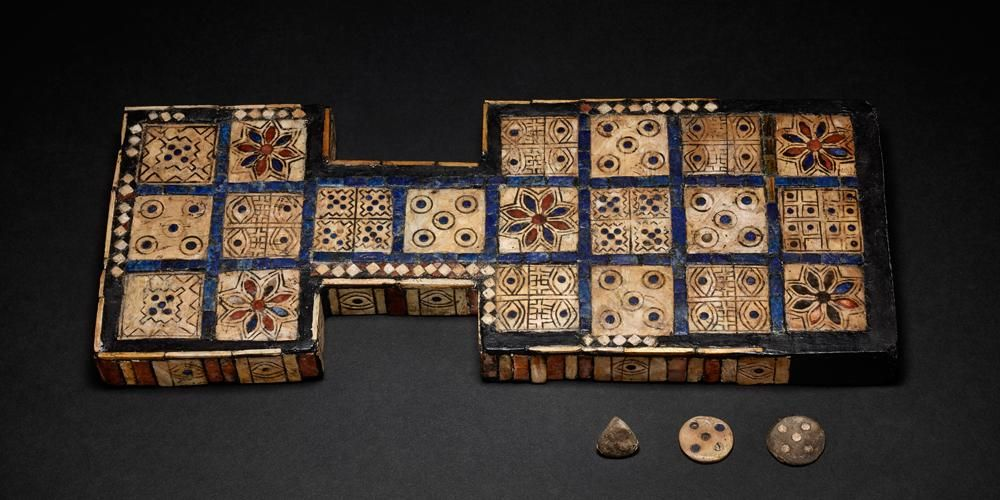
\includegraphics[width=0.7\textwidth]{Figures/Theory/royal-game-of-ur-british-museum.jpg}
    \caption{Replika hry \textit{The Royal Game of Ur} v British Museum. \cite{british_museum_2021}}
    \label{fig:royal_game_of_ur}
\end{figure}

Dále by se do této kategorie daly zařadit i velmi oblíbené \textbf{Šachy}, které zdánlivě provází lidstvo už od počátků. Jejich historie sahá do roku 400 př. n. l., kdy vznikla keltická hra \textit{Tafl}. Jednalo se o asymetrickou hru, ve které se jeden hráč snažil utéct se svým králem, začínajícím hru ve středu šachovnice, zatímco druhý hráč se snažil krále chytit. Historici se domnívají, že tato verze byla v Indii 6. století našeho letopočtu převzata a pozměněna ve hru \textit{Chaturanga}. Během let její popularita rostla a rozšířila se do celé Asie a nakonec i do Evropy. Do formy, kterou známe dnes, se šachy dostaly právě v Evropě až v 16. století. \cite{chess_com_2023}

Už takhle brzy tedy můžeme zaznamenat dodnes využívané herní principy: herní pole složené z políček, po kterých se hráči pohybují podle hodů kostkou, a cíl hry, kterým je dosažení určitého cíle na herním poli. \cite{attia_2018}

\subsection{Vývoj deskových her}
\label{subsec:development}

V období od 18. století se deskové hry stávaly více populárnějšími, s čímž se také zvedal zájem o jejich vývoj. Hry byly komplexnější a jejich tvorba se stala výdělečným odvětvím.

Jako jedna z prvních vývojářek deskových her je považována Američanka Elizabeth Magie, která v roce 1903 vytvořila hru \textit{The Landlord's Game}. Hra byla zamýšlena jako nástroj k vzdělávání a varování proti riskům land grabbingu - tedy spekulací s pozemky. Hráči se v ní snažili koupit pozemky, stavět na nich domy a hotely a tím získávat od ostatních hráčů peníze. V roce 1935 Magie prodala patent na hru společnosti Parker Brothers za 500 dolarů. Ti hru přejmenovali na \textbf{Monopoly} a začali ji prodávat, což se ukázalo být velmi úspěšné. \cite{attia_2018}

\begin{figure}[H]
    \centering
    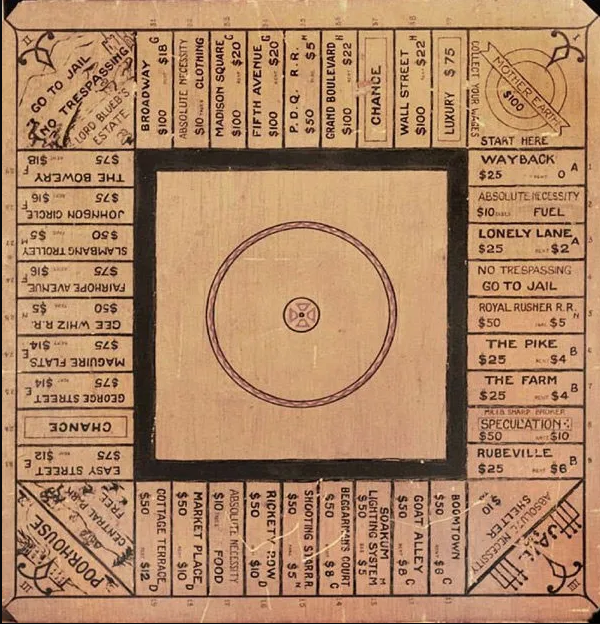
\includegraphics[width=0.3\textwidth]{Figures/Theory/landlords-game.png}
    \caption{Hra \textit{The Landlord's Game} od Elizabeth Magie. \cite{attia_2018}}
    \label{fig:landlords-game}
\end{figure}

V německu se deskové hry rozrostly tak moc, že se zde vytvořila vlastní kultura deskových her. V roce 1978 byla založena společnost \textit{Spiel des Jahres}, která každý rok uděluje cenu pro nejlepší hru roku. Tato cena se stala velmi prestižní a zvýšila zájem o deskové hry po celém světě. Zapříčinila se například za úspěch her jako \textit{Osadníci z Katanu} nebo \textit{Dixit}. \cite{attia_2018}

\subsection{Moderní směr}
\label{subsec:modern}

Kvůli vzniku a úspěchu spousty dalších her, například \textit{Carcassonne}, \textit{Ticket to Ride} nebo \textit{Risk}, se čím dál více lidí chtělo stát jejich vývojáři. V tomto jim pomohl jeden z dalších milníků - vznik Kickstarteru. Tato platforma umožňuje vývojářům prezentovat své nápady a získat na ně finanční podporu od lidí, kteří by je chtěli vidět na trhu.  \cite{attia_2018}

Díky tomu deskové hry prošly další revolucí, neboť teď tu byla možnost propagovat hru přímo hráčům, kteří by ji chtěli hrát. Velmi úspěšné projekty jako \textit{Exploding Kittens} nebo \textit{Gloomhaven} získaly na Kickstarteru miliony dolarů. Také zde začaly vznikat deskové implementace existujících videoherních titulů, jako například \textit{Darkest Dungeon: The Board Game}, \textit{The Witcher: Old World} nebo \textit{Dark Souls - The Board Game}. \cite{kickstarter}

Nemůžeme zapomenout zmínit ani giganta mezi deskovými hrami, který přinesl revoluci v herním designu - \textbf{Dungeons \& Dragons}. Tato hra, vytvořená Gary Gygaxem a Davidem Arnesonem, byla první stolní hrou, která se zaměřovala na příběh a roleplay. Hráči si v ní vytvářeli své postavy a procházeli s nimi dobrodružstvím, které jim připravoval tzv. \textit{Dungeon Master} - hráč, který hru řídil a vytvářel pro ostatní dobrodruhy příběh. Tento nápad byl tak úspěšný, že vytvořil celý žánr - \textit{tabletop RPGs} - a inspiroval spoustu dalších her, jak deskových, tak videoherních. \cite{dnd_beyond_2023}

V moderních hrách můžeme pozorovat, že se stále více zaměřují na roleplay a příběh a hlouběji implementují RPG prvky. I herní mechanismy se stávají více komplexními a vývojáři se nebojí experimentovat s novými nápady. Hry začínají být i obsáhlejší, což se projevuje v delší době hraní, větší složitosti pravidel a větším množství fyzických komponent.


\section{Definice pojmu desková a stolní hra}
\label{subsec:boardgame_definition}

V této oblasti herního designu se můžeme setkat se dvěma základními pojmy: \textit{desková hra} a \textit{stolní hra}. Tyto pojmy se často používají zaměnitelně, ale mají odlišné významy. Proto si je zde přiblížíme.

\textbf{Desková hra} (board game) je obvykle hra, jejíž hlavní součástí a neoddělitelnou komponentou je herní deska. Samotné provedení desky se může lišit, může se jednat o klasickou čtvercovou desku, nebo o jiný tvar, jako například kruhovou, hexagonální nebo jinou. Deska může být také rozdělena na políčka, která mohou mít různé vlastnosti, například barvu, číslo nebo symbol. Hra může mít také další komponenty, jako jsou karty, kostky, figurky, žetony, atd. Herní systém většinou bývá intuitivní a jednoduchý, snažící se zaměřit na širší publikum hráčů. Herní mechaniky se často točí okolo desky a ostatních fyzických komponent a neobsahují velkou míru abstrakce. Do této kategorie patří například \textit{Monopoly}, \textit{Osadníci z Katanu} nebo \textit{Carcassonne}. \cite{board_game_supply_2023}

\textbf{Stolní hra} (tabletop game) je obecnější termín, který zahrnuje všechny hry, které se hrají na stole. To znamená, že do této kategorie můžeme zařadit i hry, které nemají herní desku, jako například karetní hry, hry s kostkami, nebo hry, které se hrají pouze s papírem a tužkou. I když jsou komponenty jejich důležitou součástí, některé stolní hry si dovolují vyšší míru abstrakce herních systémů, což jim dává větší možnosti hloubky na úkor odcizení některých skupin hráčů. Toto můžeme pozorovat například u prosperujícího žánru RPG her, kam můžeme zařadit Na vlnách neznáma, \textit{Gloomhaven} nebo i výše zmíněné \textit{Dungeons \& Dragons}. \cite{board_game_supply_2023}

Pro účely této práce se budeme věnovat především deskovým hrám, ale budeme se snažit zahrnout i některé prvky stolních her, které by mohly být pro náš návrh užitečné.
\chapter{Teorie herního designu}
\label{chap:game_design}

V této kapitole jsou popsány základní pojmy herní teorie a designu, které budou sloužit jako základ pro vlastní návrh. \cite{building_blocks_of_tabletop_design_2022}


%%% section: Structure %%%

\section{Herní struktura}
\label{sec:structure}

Herní struktura je základním stavebním kamenem každé hry. Jedná se o sadu pravidel, která určují, jak se hraje, co mohou hráči dělat a jakým způsobem se hra vyhrává. Typy struktur se liší podle jejich přístupu k herním systémům a mechanikám. 

\subsection{Kompetetivní hry}
\label{subsec:structure_competitive}

Kompetetivní hry tvoří velkou část trhu s deskovými hrami. V těchto hrách se hráči snaží porazit ostatní a dosáhnout vítězství. Tyto hry můžou být symetrické, kdy všichni hráči začínají se stejnou nebo alespoň podobnou silou, nebo asymetrické, kdy mají hráči různé schopnosti a cíle. Častým problémem bývá vybalancovat hru tak, aby byla zábavná pro všechny hráče, a to i přesto, že se může stát, že jeden hráč bude mít výhodu. Dále se často stává, že hra skončí remízou. V takovém případě se může o vítězi rozhodnout buď pomocí nějakých dodatečných pravidel, nebo může skončit sdíleným vítězstvím.

Příklady: \glsref{monopoly}, \glsref{carcassonne}, \glsref{chess}, \glsref{race_for_the_galaxy}

\subsection{Kooperativní hry}
\label{subsec:structure_cooperative}

Naopak kooperativní hry se snaží hráče spojit proti společnému nepříteli nebo problému. Hráči spolupracují na dosažení cíle, který je obvykle nějakým způsobem předem daný. Velkou výhodou toho typu her je to, že odstraňují překážky, které by lidem bránily si tento typ her zahrát. Když jsou hráči spolu ve stejném týmu, dokáží vyrovnat jejich schopnosti a zkušenosti, což může novým hráčům pomoci se do hry dostat.

Kooperativní hry se dají dále rozdělovat podle různých kritérií. Například některé mohou hráče spojit v boji proti oponentovi ve formě umělé inteligence nebo sady algoritmů, zatímco jiné dávají týmu za úkol vyřešit hádanku a nemají žádného protivníka. Dalším kritériem může být, jestli hra má skryté informace, nebo jestli jsou všechny informace sdílené. Sdílení zdrojů, způsob komunikace a způsob, jakým se hra vyhrává, jsou dalšími faktory, které mohou kooperativní hru ovlivnit.

Příklady: \glsref{pandemic}, \glsref{arkham_horror}, \glsref{gloomhaven}, \glsref{forgotten_waters}


\subsection{Hry se scénářem}
\label{subsec:structure_scenario}

Tento typ her se často zaměřuje především na příběh, historickou tematiku a RPG elementy. Průběh hrou se skládá z jednotlivých epizod, které můžou být předem naplánované a navázané na sebe. Tento systém se často používá v tzv. \textit{dungeon crawlerech}, kde hráči prochází jeden dungeon za druhým. S tímto formátem je jednoduché vyměnit mapu, typy nepřátel nebo příběhové zabarvení a hráči mohou zažít více dobrodružství bez toho, aby se museli učit nová pravidla. Je to také jednoduchý způsob, jak nastavit obtížnost hry, protože každý scénář může být jiný.

Příklady: \glsref{catan}, \glsref{gloomhaven}, \glsref{pathfinder}

\subsection{Legacy hry}
\label{subsec:structure_legacy}

Legacy hry jsou speciální typ her, který se vyznačuje nenávratnými změnami, které hráči během hraní páchají na herních komponentách. Jde o změny fyzického rázu, jako je psaní na herní desku, trhání karet nebo lepení nálepek. Tyto změny mohou být způsobeny výsledkem hry, nebo mohou být součástí příběhu. Tento typ her se často zaměřuje na příběh a vývoj postav, a proto mají velmi blízko k RPG žánru. Kampaně v nich mohou trvat i několik měsíců či let, rozdělených do jednotlivých několikahodinových sezení. Jedná se o relativně nový fenomén, který se však v posledních letech začal rozšiřovat a získal si své publikum.

Příklady: \glsref{risk_legacy}, \glsref{hp_hogwarts_battle}, \glsref{gloomhaven}


%%% section: Turns %%%

\section{Pořadí a struktura tahů}
\label{sec:turns}

Se zavedením struktury přichází potřeba rozhodovat, kdy hráči mohou konat různé akce nebo kroky. Odsud vznikla myšlenka \textbf{tahu} - jednotky času, během které mohou hráči se hrou interagovat. Více tahů pak tvoří jedno \textbf{kolo}, přičemž běžné hry se skládají z několika takovýchto kol. V některých titulech se kola navíc rozdělují do několika \textbf{fází}, které většinou třídí akce do různých typů, čímž umožňují ještě větší stukturovanost herního kola. Tato pravidla se však mohou lišit podle typu hry, proto se tato sekce věnuje přiblížení několika základních typů struktury tahů.

\subsection{Kolo s pevným pořadím}
\label{subsec:turns_fixed_order}

Jedná se o nejzákladnější typ struktury kola, kdy se pořadí hráčů určí jednou na začátku hry a od té doby zůstává neměnné. Obvykle se nějakým způsobem vybere první hráč a dál tahy pokračují podél stolu ve směru nebo proti směru hodinových ručiček (například v klasické karetní hře \textit{Prší}). Tento typ struktury je velmi jednoduchý a intuitivní, ale může být nevýhodný pro hry, kde je výhoda mít první tah, nebo chceme zajistit, aby všichni hráči měli stejný počet tahů. Toto se dá řešit zvýhodněním odstaních hráčů jinými způsoby, například herními bonusy (mana navíc pro druhého hráče v \glsref{hearthstone}), nebo tím, že budeme monitorovat, který hráč začínal, a poslední kolo se vždy dojede až k němu, i kdyby hra byla ukončena v průběhu kola (jako v \glsref{through_the_ages}, kde všichni dojedou celé kolo po tom, co jeden hráč zvítězí).

\subsection{Kolo s pořadím podle statistik}
\label{subsec:turns_stat_order}

Tento typ struktury kola se snaží vyrovnat výhody a nevýhody, které mohou vzniknout z pevného pořadí. Pořadí se v tomto případě mění podle nějakého skóre, které se během hry mění. Určující statistikou může být například počet bodů, které hráči mají (tokeny populace v \glsref{civilization}), nebo nějaké pevnější statistiky spojené se samotnými postavami. Tento systém se často používá v RPG hrách, kde se pořadí může měnit podle iniciativy postav (klasická iniciativa v \glsref{dnd}), nebo ve hrách, kde se pořadí mění podle toho, jak dobře nebo špatně se hráči daří (znevýhodnění nejlepších hráčů ve \glsref{power_grid}). Hra pak dokáže být dynamičtější a aktivně reagovat na změny, což přináší nové strategické možnosti a větší zapojení hráčů.

\subsection{Kolo s pořadím určeném v reálném čase}
\label{subsec:turns_realtime_order}

Další zajímavou možností určení pořadí je nechat hráčům volnou ruku, často omezenou nějakým časovým limitem. Je pak na rychlosti samotných hráčů, jak rychle dokážou reagovat na situaci a provést svůj tah. Silnou stránkou tohoto systému je to, že hra může být mnohem rychlejší a dynamická a často s sebou přináší vyšší úroveň soutěživosti (například u hry \glsref{dobble}). Nevýhodou je to, že může být pro některé hráče stresující a může být obtížné udržet přehled o tom, co se děje. Také se designer musí více rozmyslet, jak řešit chyby hráčů a také podvádění, které v tomto zmatku bývá častější.

\subsection{Kolo s náhodným pořadím}
\label{subsec:turns_random_order}
% TODO - najít hru, která tohle používá

Náhodný výběr figurek nebo žetonů reprezentujících jednotlivé hráče, často losované z pytlíku nebo balíčku, je skvělý způsob, jak udělat hru méně předvídatelnou. Bohužel s sebou nese i snížené možnosti strategie ze strany hráčů, takže se hodí spíše pro hry, které nemají s náhodou problém a snaží se být spíše zábavné a chaotické. V opačném případě se musí zavést nějaké doplňkové mechanismy, které hráčům umožní reagovat na náhodu a otočit ji ve svůj prospěch.

\subsection{Kolo se současným výběrem akcí}
\label{subsec:turns_action_selection_order}

Posledním typem struktury kola, který si zde přiblížíme, je kolo, kde hráči vybírají akce současně, často v tajnosti. Když jsou všichni připraveni nebo po uplynutí nějakého určeného času, se všechny akce odhalí najednou a provedou se (v \glsref{gloomhaven} si hráči nejprve zvolí své akce, ale provést je mohou, až když na ně přijde řada). Často je tady třeba také druhotná mechanika pro určení pořadí, ve kterém se akce vyhodnotí (například v \glsref{race_for_the_galaxy}, kde si hráči nejprve zvolí fáze, které chtějí hrát, a pak si v tajnosti zvolí akce, které se pak vyhodnotí v pořadí vybraných fází). Tajné vybírání akcí je vhodné pro hry, které dávají důraz na strategii a odhadování akcí soupeřů.


%%% section: Actions %%%

\section{Akce}
\label{sec:actions}

Po přiblížení variant střídání hráčů během hry je vhodné zaměřit se na to, co mohou ve hře vlastně dělat. Tím se dostáváme k \textbf{akcím}, které pomáhají jednoduše a srozumitelně definovat, co mohou hráči dělat a jakým způsobem toho mohou dosáhnout. Jedná se o atomický krok v rámci hry, příkladem může být hod kostkou, pohyb figurkou, nebo zahraní karty. Akce hře dodávají dynamiku a určují celkový pocit a atmosféru, kterou hra vytváří.

\subsection{Akční body}
\label{subsec:actions_action_points}

Častým způsobem zpeněžení akční ekonomiky je sytém akčních bodů, kdy hráči mají k dispozici určitý počet bodů, které mohou během kola utratit za různé akce. Akce samotné potom mají vždy nějakou cenu, takže hráči musí dobře zvážit, jak své body využijí. Může se jednat o reálné akční body (čtyři body za kolo v \glsref{pandemic}) nebo různé typy bodů (civilní a vojenské body v \glsref{through_the_ages}). Jednodušší možnost je definovat body implicitně, pomocí nějakého zjednodušeného pravidla (jako v \glsref{gloomhaven}, kde hráči mohou za kolo udělat přesně dvě akce). Tento systém je velmi flexibilní a umožňuje hráčům volit různé strategie.

\subsection{Omezený výběr akcí}
\label{subsec:actions_limited_actions}

Jiný způsob, jak limitovat akce, je dát hráčům na výběr z omezeného množství karet, obvykle s tím pravidlem, že když už si někdo kartu vybral, pro ostatní je pro toto kolo zamčená. Tato praktika přináší možnosti interakce přímo do samotného výběru akcí, kdy hráči musí přemýšlet nejen nad tím, co by chtěli udělat, ale také nad tím, co by chtěli, aby ostatní hráči udělat nemohli (tajný výběr jedné karty z balíčku, který se pak předá dalšímu hráči v \glsref{citadels}). V kooperačních hrách to zase umožňuje hráčům spolupracovat a plánovat své akce tak, aby se co nejvíce doplňovaly, a také přináší možné dilema, jestli si nejlepší akci vybrat pro sebe, nebo ji ponechat jinému hráči (\glsref{forgotten_waters}, kde jsou některé akce vylepšující postavu limitované).

\subsection{Pálení akcí}
\label{subsec:actions_burning_actions}

Některé hry místo ceny nebo omezování akcí mezi hráči používají jiný způsob limitace, a to přidání akcí na jedno použití. Takovéto akce mají často potenciál být mnohem silnější než běžné akce a jejich použití s sebou nese důležité rozhodnutí, kdy je nejlepší je použít. Spolu s pálením akcí se často používá i nějaký způsob, jak získat tyto akce zpět, ať už to je nějaký druh obnovení, nebo nějaký druh zisku, který je spojen s nějakým rizikem (například v \glsref{gloomhaven} si hráči mohou obnovit své akce pomocí jiných akcí). Něco podobného můžeme pozorovat i v \glsref{dnd}, kde jsou nějaké akce omezené pouze jednou za dlouhý nebo krátký odpočinek. Je však třeba dávat pozor, aby se hráči necítili, že musí své akce šetřit a raději je vůbec nepoužívali.

\subsection{Příběhový výběr}
\label{subsec:actions_story_choice}

Pro hry, které se zaměřují na příběh a vývoj postav, může být vhodné, aby hráči měli možnost volit, jakým směrem se bude příběh ubírat. Tento výběr se pak stává jednou z akcí, většinou takovou, kde je hráčům položena nějaká otázka nebo problém a jejich úkolem je vybrat si možnost, která se jim nejvíce zamlouvá (opět \glsref{gloomhaven}, který při vstupu do města vždy nabídne několik možností, jak se postavit k dané situaci). Pro tento typ her je důležité, aby se hráči cítili, že jejich volba má nějaký význam a že se příběh kvůli nim mění, což s sebou přináší další problémy ohledně toho, jak efektivně měnit svět bez nutnosti vytvoření nového obsahu, který většina hráčů nemusí vůbec zažít.

\subsection{Rozhodnutí konfliktů}
\label{subsec:actions_action_resolution}

Akce mohou být jednoznačné (tah v \textit{Šachu}, kde se všechno stane přesně tak, jak si to hráč vymyslel), ale v komplexnějších hrách bývají často nejisté, nebo spojené s nějakým druhem náhody. Přichází tedy problém, jak rozhodneme o výsledku akce.

Nejjednodušším způsobem je systém, kdy vždy vyhrává vyšší číslo. Může se jednat například o číselnou reprezentaci síly hráče (síla karty v \glsref{magic}), nebo o hod kostkou. Tento systém je velmi jednoduchý a intuitivní, ale může být nevýhodný pro hry, kde chceme, aby některé akce byly vždy úspěšné, nebo naopak vždy neúspěšné.

Jiný způsob kontroly je tzv. stat check - hráči musí porovnat nějakou statistiku své postavy s předem danou hranicí potřebnou pro úspěch. Tato kontrola se často spojuje s hodem kostky (jako v \glsref{dnd} nebo \glsref{forgotten_waters}, kde si hráči hodí na nějakou statistiku a přičtou k tomu svůj modifikátor). Pro RPG hry je toto skvělý způsob jak vyzdvihnout jedinečnost každé postavy a dát hráčům možnost se v ní projevit.

Další zajímavou obměnou je zavedení kritických úspěchů a neúspěchů. Obvykle se jedná o situaci, kdy hráči na kostce hodí nejvyšší nebo nejnižší možnou hodnotu. V klasickém \glsref{dnd} se u útoku při hodu 20 zranění zdvojnásobí, zatímco při hodu 1 útok úplně mine. Souboji to pak dodává větší napětí a potenciál dramatických a často zábavných zvratů.


%%% section: Movement %%%

\section{Pohyb po herním poli}
\label{sec:movement}

Už první deskové hry jako \glsref{senet} nebo \glsref{mahjong} (sekce \ref{subsec:beginnings}) měly \textbf{pohyb} po herním poli jako centrální herní mechaniku. Způsob, jakým hráči pohybují svými figurkami má velký vliv na to, jakou atmosféru hra nabízí a jaké strategické možnosti hráčům dává. Následující sekce popisuje několik různých mechanik, které jsou s pohybem spojené.

\subsection{Rozdělení herního pole}
\label{subsec:movement_tessellation}

Herní pole deskových her mnohdy představuje velký prostor, u komplexnějších her se může jednat klidně o celé kontinenty nebo až galaxie. Aby se hráči v tomto prostoru lépe orientovali, bývá pole často rozděleno na nějaké menší části, které se dají pohodlněji zobrazit na herní desce.

Nejjednodušším způsobem rozdělení je \textbf{jednodimenzionální rozdělení}, které je reprezentováno jednou cestou, kterou hráči během hry musí projít. Cesta se může dále rozštěpit na různé větve, které můžou být zkratky nebo mohou vést k různým cílům (hlavní cesta a zkratky nebo skluzavky ve hře \glsref{snakes}).

Pokud nám jedna cesta nestačí, můžeme přejít na \textbf{dvoudimenzionální rozdělení}, kde se hrací plocha rozdělí na mřížku. Z pravidelných tvarů se nejčastěji používají čtverce (např. \glsref{chess}) nebo hexagony (např. \glsref{gloomhaven}), přičemž každý má své vlastní výhody a nevýhody. U čtverce musíme myslet na to, jestli umožníme diagonální pohyb, protože podle pythagorovy věty by tento pohyb měl být $\sqrt{2}$ ($1.41$) krát delší než pohyb po straně. Hexagony jsou v tomto ohledu příjemnější, neboť všech šest směrů má stejnou vzdálenost, ale zase se je těžší je reprezentovat v klasické mřížce. 2D prostor můžeme rozdělit také do nepravidelných tvarů, často reprezentující terén nebo státy (části mapy v \glsref{diplomacy}).

Další možností pak je \textbf{třídimenzionální rozdělení}, kdy se hrací plocha rozčlení do několika vrstev, které se mohou překrývat nebo být oddělené. Rozdělení do výšky můžeme docílit buď pomocí indikátorů úrovně nebo různých pater hracích ploch, které můžeme fyzicky postavit nad sebe.

\subsection{Pohyb podle hodu kostkou}
\label{subsec:movement_roll_movement}

První způsob určení pohybu, který deskové hry adaptovaly, je pohyb podle nějakého náhodného čísla. Může se jednat o kostku (\glsref{monopoly}), ruletu (\glsref{party_alias}) nebo karty (\glsref{candyland}). Čistá náhoda však může zmírnit taktické plánování, proto můžeme zavést nějaký druh modifikátoru, který hráčům umožní ovlivnit výsledek (například bonusy k rychlosti v \glsref{formula_d}).

\subsection{Pohyb podle ceny}
\label{subsec:movement_cost_movement}

Jiná možnost je nacenit každé políčko na herní desce a dát hráčům nějakou měnu, kterou mohou za pohyb utratit. Často se používá ve válečných hrách, kde vyšší cena políčka může znamenat nepříznivé terénní podmínky a dostupné množství měny zase rychlost jednotlivých figurek (\glsref{third_reich}). Hráči pak mají více možností a musí zvažovat nejen to, kam své figurky posunou, ale také to, kudy bude nejlepší projít.

\subsection{Odhalování terénu}
\label{subsec:movement_map_reveal}

Dynamická změna herního pole se často používá ve hrách zaměřených na průzkum a objevování. Hráči se pohybují po herní ploše a postupně odhalují nové části, na které musí reagovat. Odhalovat se můžou buď jednotlivá pole (\glsref{lovci_pokladu}), nebo celé části mapy (\glsref{gloomhaven}).

Herní pole však nemusíme jen zvětšovat, ale můžeme ho i odebírat. S podobnou mechanikou se můžeme setkat u dětské hry \textit{Židličky}, ale v kontextu stolních her může jít o opravdové odstraňování herních polí (postupné odstraňování polí v \glsref{isolation}), nebo jen o pouhou limitaci možností, které hráči mají (snižování možností na nové železniční spoje v \glsref{ticket_to_ride}).

\subsection{Více map}
\label{subsec:movement_multiple_maps}

Aby byl herní svět co nejvíce rozmanitý, můžeme vytvořit více map, které se mohou během hry měnit. Může se jednat o jednotlivé lokace, které jsou spojené cestami (propojení mezi hlavní a podzemní mapou v \glsref{iron_dragon}), nebo jsou všechny umístěné ve světě hry a odemykají se postupně (odhalování nových lokací podle příběhového postupu v \glsref{gloomhaven}). Zakomponování více lokací se spojujícími cestami může být dobrý způsob, jak hráčům dát možnost volby a také v nich navodit pocit, že jejich postavy jsou součástí nějakého většího světa.


%%% section: End %%%

\section{Konec hry}
\label{sec:end}

Samotný herní systém může být sebelepší, ale pokud nemá jasně definovaný konec, může se stát, že hráči si po jejím ukončení odnesou jen zklamání. Proto je důležité, aby hra měla pečlivě vymezený \textbf{cíl} a způsob, jakým se dá dosáhnout. Závěrná sekce analýzy herního designu je tedy zaměřena na to, jaké cíle se u deskových her vyskytují.

\subsection{Body vítězství}
\label{subsec:end_victory_points}

Většina moderních her využívá nějakou verzi systému bodu vítězství. Jedná se o velmi flexibilní mechaniku, kdy hráči během hry sbírají jednu nebo více surovin, které se po ukončení hry převedou na body a určí vítěze. Vítězné body je možné udělovat mnoha způsoby.

První z nich je získání bodů \textbf{ze stavu hry}. Hráči často mají předem určené cíle a snaží se s herním stavem manipulovat tak, aby je to co nejvíce odráželo. To, kdy se budou body počítat, může také ovlivnit ideální strategii. V některých hrách se body počítají až na konci hry (\glsref{agricola}), jinak se ale mohou počítat po intervalech (třikrát za hru v \glsref{el_grande}), po určitých akcích hráčů (hráč zahraje speciální kartu počítání bodů v \glsref{expanse}), nebo náhodně (vylosování speciální karty z balíčku v \glsref{airlines}).

Jiný přístup je odměňovat hráče body \textbf{za určité akce}. Dobrým příkladem je hra \glsref{race_for_the_galaxy}, kde hráči získávají body za tažení různých karet nebo prodej produktů. Kromě toho hra obsahuje i složitější mechanismus úkolů, které jsou buď sdílené nebo si odměnu může vzít jen první hráč, který je splní. Tyto úkoly slouží mimo jiné i k nenásilnému navádění hráčů k různým strategiím, které by možná jinak nezkusili.

Zajímavou dynamiku můžeme do hry přinést také tím, že umožníme vítězné body nejen získat, ale i ztratit. Pokud je možné o všechny body přijít, riskujeme, že se hráči budou soustředit spíše na to, aby shodili vedoucího hráče než aby se snažili sami vyhrát (tohle je velký problém například v karetní hře \glsref{munchkin}). Lepší bývá implementovat mix trvalých a dočasných bodů, což hráčům přidá možnost strategií, ale zároveň omezí potenciální zneužití (dobrým příkladem je \glsref{kemet}).

\subsection{Závod}
\label{subsec:end_race}

Velmi intuitivní způsob, jak určit vítěze, je závod. Hráči se snaží co nejrychleji dosáhnout nějakého cíle, který je předem určen. Ten může být buď fyzický, jako je dosažení určitého pole na herní desce (\glsref{snakes}), nebo může být abstraktní, jako dosažení určitého počtu bodů (\glsref{catan}).

\subsection{Vyčerpání zdrojů}
\label{subsec:end_resource_depletion}

Další možností je zahrnout do hry nějaký druh zdroje, který se postupně vyčerpává. Hra je pak přirozeně vedena k očekávanému konci a hráči si mohou sami určit, jak dlouho může trvat. Příklady můžeme vidět ve hře \glsref{through_the_ages}, kde hra končí, když v bance dojdou peníze, nebo v \glsref{race_for_the_galaxy}, kde hráči získávají body z limitovaného množství a konec hry nastane, když body dojdou.

\subsection{Kooperativní cíle}
\label{subsec:end_cooperative_goals}

V kooperativních hrách je vhodné vymyslet jiný způsob, jak ukončit hru - místo soutěžení o vítězství můžeme hráče motivovat ke společnému dosáhnutí nějakého cíle. Společný cíl může mít různé podoby, ať už poražení společného nepřítele (vyléčení všech nemocí v \glsref{pandemic}), dosažení nějakého bodového maxima (zabrání dostatečného množství pevností v \glsref{dune}) nebo splnění nějakého úkolu (zničení Jednoho prstenu v \glsref{war_of_the_ring}). Týmové cíle podporují spolupráci a komunikaci, musíme si ale dávat pozor, aby se hráči necítili, že nemají na herní dění dostatečný vliv.


%%% section: App %%%
\section{Podpůrné aplikace}
\label{sec:apps}

V posledních letech se stále více vývojářů stolních her snaží využít moderní technologie, ať už ve formě mobilních aplikací, nebo webových stránek. Tyto aplikace mohou sloužit k různým účelům, jako je například pouhé zobrazení pravidel, ale může jít i o stěžejní část hry. Tato sekce rozebírá fáze propojení mezi hrou a aplikací a možnosti, které se s tím pojí. \cite{corvus_belli_2023}

\subsection{Stupně integrace}
\label{subsec:apps_app_integration}

Neboť jsou podpůrné aplikace relativně novým fenoménem, po celou historii vývoje byla většina stolních her \textbf{plně fyzická} záležitost. I dodnes se tato tradice stále drží, spousta nově vyvinutých her se neopírají o žádnou podpůrnou aplikaci a všechnu administrativu nechávají čistě na hráčích. Nejde jen o samotný herní plán, figurky nebo karty a kostky, ale také o pravidla, která jsou většinou tištěná na papíře a přiložená k hře. Příkladů takovýchto her je mnoho, například \glsref{carcassonne}, \glsref{ticket_to_ride} nebo \glsref{catan}.

I u plně fyzických her je však občas přínosné, aby jejich pravidla nebo nějaké další podpůrné materiály byly dostupné i v digitální podobě. Důvodem může být to, že hráči nepotřebují mít všechna pravidla přístupná neustále a jejich digitalizace umožní jednodušší vyhledávání a možnost jejich postupného odhalování. V takovém případě může být vhodné vytvořit \textbf{digitální verzi pravidel}, která bude dostupná na internetu nebo jako aplikace. Tato verze může být vytvořena buď v podobě PDF souboru, jako webová stránka, nebo jako aplikace pro mobilní zařízení. Jako příklad můžeme uvést karetní hru \glsref{munchkin}, která má jednoduchý výčet pravidel obsažený v balení, ale také má oficiální webové stránky, kde mohou hráči najít hlubší vysvětlení pravidel a návody na hraní.

V jiných případech může aplikace sloužit jako \textbf{administrativní doplněk} ke hře, který hráčům pomáhá s organizací, kterou by jinak bylo obtížné a pracné udržovat na papíře. Může jít o držení informací o herním stavu, počítadla bodů a životů, nebo o monitorování stavu inventáře, případně nějaké herní měny. Aplikace zde stále není důležitou součástí hry, ale jen umožňuje zjednodušit tyto rutinní činnosti, aby se hráči mohli soustředit na samotnou hru. Příkladem může být neoficiální aplikace \textit{Gloomhaven Secretariat}, která usnadňuje administrativu v kooperativní hře \glsref{gloomhaven}.

Největší míru integrace můžeme vidět v deskových hrách, které jsou \textbf{zcela závislé na aplikaci}. V takovýchto hrách je aplikace nejen doplňkem, ale stěžejní součástí hry, která spravuje herní plán, pravidla a jiné herní mechaniky. Dále se tímto způsobem dá velmi jednoduše a efektivně připojit příběh, který může být ozvláštněn automatickým čtením, zvukovými efekty nebo animacemi. Příkladem může být hra \glsref{mansions_of_madness}, kde je aplikace nejen zdrojem pravidel, ale také generuje herní plán, spravuje nepřátele a vytváří silnější atmosféru.

\subsection{Přínosy aplikace}
\label{subsec:apps_app_benefits}

Prvním přínosem, který byl zmíněn v předchozí sekci, je možnost zjednodušení administrativy. Hlavní benefit spočívá v tom, že hra samotná se postará o monitorování zdrojů nebo počítání bodů. Tímto způsobem se hráči mohou soustředit na samotnou hru a nemusí se starat o to, jestli všechno správně počítají. Hráči mohou také mít jednodušší přístup k informacím, které by jinak byly obtížně dostupné, jako například aktuální stav inventáře, zdrojů nebo bodů ostatních spoluhráčů. Digitalizace pravidel také plní podobnou funkci, hráči nemusí mít všechna pravidla stále při ruce, ale mohou si je kdykoliv vyhledat.

Propojení s aplikací může být také příjemný způsob, jak hru trochu oživit a poskytnout hráčům záživnější zážitek. Vývojáři mohou využít zvukových efektů, jako může být hudební a ambientní podkres, nebo například dynamické zvuky řevu, když se na hráče připravuje zaútočit nepřítel. Hlasové vyprávění může být také velmi přínosné, pokud se jedná o hru s příběhem, který se postupně odhaluje. Hráči pak mohou příběh zažívat spolu nezávisle na jejich čtenářských schopnostech. Na posílení herního zážitku může být také využito obrázků nebo animací. Když se desková hra musí držet pevného rozpočtu, přidání složitých herních komponent nebo detailních figurek může být nákladné, zatímco digitální obsah může být vytvořen za mnohem nižší cenu.

V příběhových hrách může být problém zajistit, aby klíčové informace nebo zvraty byly odhaleny ve správném pořadí a správný čas. U příběhu tištěného na papír jako součást pravidel existuje risk, že hráči si příběh omylem přečtou dřív, než by měli, a přijdou tak o možnost překvapení. Aplikace může tuto situaci řešit tím, že bude informace odhalovat postupně a hráči se nemusí bát, že něco přeskočili nebo zjistili dříve, než to bylo zamýšleno. Takovýto příběh v kombinaci s hlasovým vyprávěním a výstižnými obrázky může být velmi poutavý a zvednout kvalitu herního zážitku.

Deskové hry, které trvají přes několik sezení (\textit{legacy hry}, zmíněny v kapitole \ref{subsec:structure_legacy}) mohou mít problém s udržením konzistence herního stavu mezi jednotlivými sezeními. Za pomocí aplikace mohou vývojáři poskytnout hráčům praktický a pohodlný způsob, jak si rozehranou hru uložit. Tímto způsobem se hráči nemusí strachovat, že by něco zapomněli, a když se ke hře znovu vrátí, budou mít vše přichystané tak, jak minule skončili.

Posledním přínosem, který aplikace může přinést, je možnost rozšíření hry. V případě fyzických rozšíření je potřeba nejen vymyslet nový materiál, ale i zajistit jeho výrobu a distribuci. Digitální rozšíření může být vytvořeno za mnohem nižší cenu a může být distribuováno přímo přes webové stránky nebo aplikaci. Vývojáři pak mají možnost pružně reagovat na zpětnou vazbu od hráčů a mohou také vytvářet obsah, který by byl jinak příliš nákladný na výrobu.

\subsection{Překážky a problémy}
\label{subsec:apps_app_problems}

Přestože může být propojení s aplikací velmi přínosné, může také přinést několik problémů, které je třeba zvážit. Prvním z nich je, že i přes to, že se většina lidí již umí pohybovat v digitálním prostředí, stále existují skupiny, které mají s používáním technologií problém. Může jít o starší lidi, kteří nemají s technologiemi mnoho zkušeností, nebo o osoby s nějakým druhem postižení, které jim znesnadňuje tuto práci. Proto vývojáři musí během návrhu aplikace myslet na to, jak ji udělat co nejpřístupnější pro co nejširší skupinu lidí. Vhodné může být i udělat aplikaci přístupnější na více platformách nebo umožnit její použití i bez připojení k internetu. Aplikace může být také obohacena o možnosti nastavení vizuálu a také jazyků, aby podporovala širokou míru uživatelů.

Dále je důležité produkt s aplikací dobře nacenit. Některé aplikace s sebou mohou přinést další výdaje, které by se u čistě fyzické hry nevyskytly. Desková hra je obvykle jednorázový nákup, zatímco aplikace může vyžadovat pravidelné platby nebo nákup dalšího obsahu. Aplikace potřebuje podporu a údržbu, což může být nákladné, a vývojáři musí být také schopni zajistit, že aplikace bude stále dostupná a bude fungovat i na nových zařízeních. Proto většina deskových her využívajících aplikaci dodává aplikaci zdarma, nebo přesněji zahrnutou v ceně hry. Na druhou stranu je však nutno zmínit, že aplikace může výrobní cenu hry i snížit, proto je třeba zvážit, zda se náklady na vývoj a údržbu vrátí v prodeji.

S modernizací obchodu s deskovými hrami se však začínají ozývat také obavy o to, zda je vůbec vhodné, aby deskové hry využívaly aplikace. Někteří hráči mají obavy, že se hry příliš digitalizují a ztrácejí tak svůj původní charakter. Ve dnešním světě plném obrazovek se mnozí hráči chtějí odpojit od digitálního světa a desková hra, která se až moc opírá o aplikaci je může odradit. Vývojáři tedy musí najít rovnováhu mezi tím, aby aplikace byla přínosná, ale zároveň aby nebyla příliš nápadná a neodváděla pozornost od samotné hry.

I přes tyto problémy je však možné, že v budoucnosti bude většina deskových her využívat nějakou formu aplikace. Dobře navržená podpůrná aplikace dokáže herní zážitek zlepšit a obohatit, pokud jsou vývojáři při jejím návrhu pečliví a myslí na to, jakým způsobem bude aplikace přínosná pro hráče.


%%% section: Psychology %%%

\section{Psychologie deskových her}
\label{sec:psychology}

// TODO
\chapter{Analýza existujících her}
\label{chap:game_analysis}

Tato kapitola se zaměřuje na analýzu několika existujících deskových her, které poslouží jako inspirace pro vlastní návrh modelové hry. Rozebrány budou klady i zápory těchto her, co je dělá zajímavými, co je na nich dobré a co by naopak bylo třeba změnit. Analýza se bude zaměřovat především na herní principy, které byly uvedeny v předchozí kapitole \chapterref{chap:game_design}.


%%% Forgotten Waters %%%

\section{Na vlnách neznáma}
\label{sec:forgotten_waters}

\glsref{forgotten_waters} (anglicky \textit{Forgotten Waters}) je kooperativní desková hra pro 3 až 7 hráčů, kterou vydalo v roce 2020 vydavatelství Plaid Hat Games. Hra je zasazena do fantasy světa, kde hráči přebírají role pirátů, jejichž úkolem je spolupracovat, aby úspěšně splnili sen jejich kapitána. Každá z postav má však své vlastní cíle, které jsou reprezentovány vývojem postavy a jejími schopnostmi. Důležitou součástí hry je webová aplikace, která poskytuje hudební a zvukové efekty, včetně hlasového vyprávění, které hráče provází příběhem a vytváří tak atmosféru hry. \cite{forgotten_waters}


\subsection{Herní systém}
\label{subsec:fw_gameplay}

Z pohledu herní struktury tato hra jednoznačně spadá do kategorie kooperativních her \chapterref{subsec:structure_cooperative}, je však obohacena i o prvky scénářových \chapterref{subsec:structure_scenario} a legacy her \chapterref{subsec:structure_legacy}. Před samotnou hrou si hráči vyberou, pod kterým kapitánem budou sloužit jako posádka, což je v podstatě abstrakce nad pouhým vybráním herní kampaně, která obsahuje předpřipravený scénář, včetně herní mapy a příběhu, kterým budou hráči procházet. Samotná hra pak spočívá v cestování mezi lokacemi a potýkání se s událostmi, které tyto lokace nesou. Kampaň je rozdělena do několika částí, mezi kterými jsou hráči vybídnuti, aby si hru uložili a pokračovali v ní později. Jednotlivé části mohou trvat několik hodin, pokud však hráči chtějí, kampaň jde odehrát během jednoho dlouhého sezení. Herní komponenty se hrou však přímo neznehodnocují, s jedním balením je možné odehrát libovolný počet kampaní.

Lokace se ve hře vybírají pomocí pohybu lodi po mapě tvořené hexagony. Podle scénáře jsou některé hexagony předem určené, jiné jsou prázdné a když na ně hráči stoupnou, umístí místo nich náhodně vylosovanou lokaci. Herní pole je tedy rozděleno dvoudimenzionálně a mění se dynamicky \chapterref{subsec:movement_map_reveal} podle postupu posádky. Pohyb lodi je ovlivněn hodem hráče, který si vybral, že ji bude toto kolo řídit. Podle jeho úspěšnosti se loď posune u určitý počet polí, pohyb je tedy náhodný \chapterref{subsec:movement_roll_movement} s přidanými modifikátory.

V rámci lokace je hráčům představeno několik možností, které si může vybrat buď několik lidí, nebo jsou přístupné pouze prvnímu z nich \chapterref{subsec:actions_limited_actions}. Některé z nich jsou také povinné - musí si je vybrat alespoň jeden hráč. Tyto možnosti jsou reprezentovány jako vytištěný seznam akcí na stránce knihy, která je součástí balení. Výběr akcí probíhá v pořadí iniciativy, která je reprezentovaná stupnicí věhlasu, jde tedy pořadí podle jisté statistiky \chapterref{subsec:turns_stat_order}. Samotné vyhodnocování probíhá v pořadí od první akce po poslední tak, jak jsou na stránce vytištěny.

Co se týče konce hry, ten je určený předem připraveným scénářem. Každá část končí nějakou událostí, která se vyvolá po dokončení lokace. Po dokončení všech částí hry je dokončen i příběh a následuje příběhový epilog, vyhodnocený podle toho, jak se hráči během hry chovali. Jde tedy o příklad ukončení na základě splnění kooperativního cíle \chapterref{subsec:end_cooperative_goals}. Na závěr hry však ještě probíhá vyhodnocení příběhu jednotlivých postav, které v průběhu hry získávají body souhvězdí, které následně určují, jakým způsobem se příběh postavy vyvine. Jedná se tedy o ukázku konce hry na podle bodů vítězství \chapterref{subsec:end_victory_points}.


\subsection{Fyzické komponenty}
\label{subsec:fw_components}

\gameref{Na vlnách neznáma} svůj herní systém podporuje několika fyzickými komponenty, které jsou součástí balení hry. Ty nejdůležitější z nich jsou přiblíženy níže.

\subsubsection*{Herní deska}
\label{subsubsec:fw_comp_board_and_book}

Herní deska je tvořena hexagonálním polem, které reprezentuje moře, po kterém se hráči pohybují. Na tuto prázdnou šablonu se umisťují hexagonální žetony navigace, které představují místa, kterými hráči proplouvají. Když hráči plují přes prázdné pole, náhodně vylosují žeton, který na toto pole umístí, což dodává hře pocit, že v ní opravdu prozkoumávají neznámé moře. Jednotlivé žetony navigace mají své vlastní identifikační číslo, které přes aplikaci odkáže hráče na příslušnou stránku v knize lokací.

Kniha lokací je příručka, která obsahuje všechny lokace, které mohou hráči navštívit. Každá lokace má svou vlastní stránku, na které je popsána, včetně možností, které na ní hráči mají. Na levé straně jsou vždy vytištěné jednotlivé akce, na které si hráči během kola postaví své figurky a dále s těmito akcemi pracují. Na pravé straně je vytištěný tematický obrázek, který hře dodává atmosféru.

\subsubsection*{Karty}
\label{subsubsec:fw_comp_cards}

Většina ve hře karet reprezentuje předměty, které mohou hráči získat a použít. Dělí se na poklady, které hráči získávají různými způsoby během hry, a příběhové karty, které se vztahují k příběhu postav. Karty přinášejí bonusy ke schopnostem, které postavy mohou využít, a také mohou nést složitější bonusy, které jsou ve zkratce popsané na kartě. Jedná se o jednoduchý způsob, jak hráčům umožnit jedinečný vývoj jejich postav, který je zároveň snadno zpřístupněný a přehledný.

\subsubsection*{Postavy a role}
\label{subsubsec:fw_comp_roles}

Jako posádka lodi si hráči před začátkem hry rozdělí role, o jejichž povinnosti se musí postarat. Spolu se svou rolí dostanou i list nebo desku, která slouží jako počítadlo pro různé statistiky, které budou hlídat. Jedná se o následující role:

\begin{itemize}
    \item \textbf{Lodní písař}: Stará se o lodní deník.
    \item \textbf{Kormidelník}: Hlídá věhlas, který určuje iniciativu při výběru akcí.
    \item \textbf{První důstojník}: Hlídá nespokojenost a počet členů posádky.
    \item \textbf{Bocman}: Kontroluje stav trupu - pokud se loď potopí, hra končí.
    \item \textbf{Bednář}: Hlídá lodní zásoby.
    \item \textbf{Dělostřelec}: Obsluhuje lodní děla, která se využívají především v soubojích.
    \item \textbf{Pozorovatel}: Hlídá průběh příběhu.
\end{itemize}

Pomocí takovéhoto rozdělení rolí mezi hráče je zajištěno, že se všichni hráči budou muset podílet na řízení lodi, a zároveň se také zamezí tomu, aby se některé činnosti opakovaly.

Samotné postavy také mají své vlastní deníky. Tyto deníky slouží jako záznamník pro vývoj postavy, který je reprezentován body souhvězdí, které postava získává během hry. Po konci příběhu se podle těchto bodů vyhodnotí, jaký osud postavu potkal. Kromě těchto příběhů a jejich potenciálu na získávání schopností různé úrovně se však postavy moc neliší.

\subsubsection*{Kostky}
\label{subsubsec:fw_comp_dice}

Pro vyhodnocování úspěšnosti akcí se ve hře používají dvanáctistěnné kostky, které se hází vždy, když je třeba určit výsledek zkoušky dovednosti. Když si hráč háže například na sílu, k výsledku hodu kostkou přičte svou vlastní hodnotu síly a případně bonusy, které mohl získat z karet. Výsledek pak porovná s obtížností úkolu, kterou určuje scénář.

Zpestření hodů zajišťují speciální žetony, které upravují výsledek hodu. Jedná se o žetony neštěstí, při kterých si hráč musí hodit znovu a počítat si horší výsledek, a žetony přehození, které naopak umožňují ze dvou výsledků počítat ten lepší. 

\subsubsection*{Figurky}
\label{subsubsec:fw_comp_figures}

\gameref{Na vlnách neznáma} nepoužívá přímo figurky, ale volí levnější variantu - tzv. standees, ilustrace vytištěné na kartonu, které se postaví do plastových stojanů. Tyto standees reprezentují jak postavy v rámci lokace, tak i samotnou loď na herním plánu. Jednoduchost tohoto způsobu umožňuje snadnou reprezentaci postav a zároveň snižuje náklady na výrobu hry.


\subsection{Podpůrné aplikace}
\label{subsec:fw_apps}

Hlavní funkcionalitu, kterou aplikace přináší, je průvodce příběhem. Při vstupu si hráči zvolí kampaň, kterou chtějí hrát, načež jim aplikace přehraje úvodní dialog a pokud je to potřeba, krok po kroku jim ukáže, jak si mají herní desku a ostatní komponenty připravit. Dále aplikace slouží jako knihovna informací. Každý záznam, který hráčům ukazuje, má svůj třímístný kód, pomocí jehož hráči mohou na záznamy přistupovat. Tento přístup poskytuje vývojářům velkou flexibilitu v tom, odkud mohou hráči kódy získávat. Může jít o pouhé uvedení lokace (jak již bylo výše zmíněno, každá lokace má svůj odpovídající kód), krátkou anekdotu po získání nového předmětu nebo i o příběhový výsledek nějakého rozhodnutí. Jako vedlejší funkci aplikace také přináší hudební a zvukové efekty, které hru doplňují a vytváří kýženou atmosféru. \cite{fw_crossroads_app}

Nově také vznikla oficiální webová aplikace, která umožňuje hru hrát plně online. Na stránkách je možné si založit herní místnost, do které se mohou připojit ostatní hráči. Během hry jsou pak digitalizovány všechny komponenty, které jsou potřeba k hraní, včetně herní desky, knihy lokací, karet a počítadel pro jednotlivé role. \cite{fw_remote_app}

\subsection{Herní pravidla}
\label{subsec:fw_rules}

Pravidla hry \gameref{Na vlnách neznáma} jsou přiložena jako součást balení, jsou však přístupná i v digitální formě na stránkách vydavatele. Hned ze začátku jsou hráči seznámeni s důležitostí webové aplikace a je jim předložen odkaz, přes který se na ni dostanou. Následně je ve zkratce uveden a shrnut veškerý herní materiál, který je v balení obsažen, a složitější komponenty jsou vyobrazeny nákresem s popisky klíčových částí.

Hlavní část pravidel je věnována popisu postupu na přípravu hry a průběhu jednotlivých kroků. Příprava je rozepsána do očíslovaných kroků a doplněna o ilustrace, které hráčům usnadňují orientaci. Následně je hráčům vysvětleno, jak je rozděleno kolo a jak fungují akce v něm. Dále jsou také přiblíženy jednotlivé postavy, jejich dovednosti a zkoušky, které se k nim vztahují. Na závěr jsou hráči seznámeni s tím, jak může hra skončit, ať už pozitivně či negativně, a jak se hra ukládá, pokud se rozhodnou ji hrát v oddělených sezeních. Jako zajímavý bonus na konci pravidel je přiložen generátor pirátských jmen, který hráčům pomocí dvou kostek umožní vygenerovat si jméno pro svou postavu.


%%% Dungeons & Dragons %%%

\section{Dungeons \& Dragons}
\label{sec:dungeons_and_dragons}

Obrovský vliv, který měla revoluční RPG hra \glsref{dnd} na vývoj stolních her, už byl zmíněn výše. Tato hra je však také zdrojem inspirace pro mnoho deskových her, které se snaží přenést některé z jejích prvků do stolního prostředí, a rozšířit tím svou potenciální hráčskou základnu. Tato sekce se zaměřuje na analýzu prvků, které byly převzaty z \dnd{} do jiných her. Oproti jiným hrám, které jsou v této práci rozebrané, je však \dnd{} mnohem komplexnější a množství jeho herních mechanik je také mnohem větší, proto se tato sekce bude držet spíše herních systémů a mechanik, které jsou popsány ve výše zmíněné kapitole \textit{\nameref{chap:game_design}}.


\subsection{Herní systém}
\label{subsec:dnd_gameplay}

Prvně je třeba zmínit, že \dnd{} se nedrží klasické symetrické struktury, kterou většina stolních her využívá. Hra je založena na asymetrickém systému, kde jeden z hráčů, označovaný jako \textit{Dungeon Master} (DM) nebo vypravěč, má na starosti vytváření a řízení celého světa, včetně všech postav, které v něm žijí. Ostatní hráči, v tomto světě následně hrají své vlastní postavy a dělají za ně rozhodnutí, stěžejní částí herního zážitku je tedy \textit{roleplay}. Tento systém je základem pro všechny ostatní mechaniky, které jsou v této hře používány. Z tohoto popisu se může zdát, že hráči a DM soupeří o jakousi výhru, ve skutečnosti však spolupracují na vytváření příběhu, který je pro všechny zúčastněné zábavný. Tatu skutečnost z \dnd{} dělá nejen pouhou stolní hru, ale prostředek pro kooperativní vyprávění příběhů.

Svou strukturou je \dnd{} ukázkovým příkladem legacy hry \chapterref{subsec:structure_legacy}, neboť běžná kampaň může trvat až roky a z pohledu ničení herních komponent se tato charakteristika odvíjí od konkrétní kampaně a také kreativity DM a ostatních hráčů. Je zřejmý také strukturální vliv scénáře \chapterref{subsec:structure_scenario} -- pro hráče je přístupná spousta předpřipravených scénářů a kampaní, kterými se DM může řídit, ať už jde o oficiální příběh od vývojářů nebo o neoficiální práci některého z mnoha fanoušků, tvořící pro hru další obsah. Hráči se však příběhu nemusí držet, pokud nechtějí, neboť volnost herních mechanismů dává velkou flexibilitu v improvizaci a nečekaných zvratech, které často nečeká ani sám vypravěč. Ve své podstatě se také jedná o kompetetivní hru \chapterref{subsec:structure_competitive}, i když během roleplaye a herních zvratů se může jednoduše stát, že se některé z postav obrátí proti sobě a je na hráčích, jak tyto konflikty vyřešit. Tyto konflikty by však měly zůstat pouze v mezích herního světa a nevnášet neshody mezi samotné hráče.

I přes to, že příběhové sekce a částí více zaměřené na roleplay nemají téměř žádnou strukturu, během souboje je struktura relativně pevná, samozřejmě s výjimkami. Před soubojem si všechny postavy i nepřátelé hodí na iniciativu, k výsledku si přičítají své vlastní bonusy a výsledné číslo určí pořadí kola, jde tedy o určení pořadí podle statistiky \chapterref{subsec:turns_stat_order}. Ve svém kole má poté hráč přesně určená pravidla, na to, jaké akce může provést. Obvykle se jedná o pohyb, akci (útok zbraní nebo seslání kouzla) a bonusovou akci (interakci s předmětem, vytasení zbraně nebo speciální kouzla), přičemž hráč si může vybrat v jakém pořadí tyto akce provede, pokud vůbec. 

Co se týče pohybu, herní pole je obvykle rozděleno na hexagony, i když přesný vzhled mapy záleží čistě na DM. Po herním poli se hráči mohou pohybovat ve svém kole, vzdálenost, kterou urazí je zapsána v jejich deníku postavy. Mají také možnost sprintovat, což jejich rychlost zdvojnásobí, za cenu spálení akce. Pravidlem také bývá, že akce by měly dávat z prostorového pohledu smysl, například že by se postavy neměly v boji přeskakovat ani střílet po nepřátelích, když jim stojí v cestě jejich spojenci. Opět ale záleží na rozhodnutí hráčů.

Samotné souboje jsou řešeny pomocí kostek. Každá zbraň má svůj vlastní druh kostky, který se hází, když se s ní útočí. Hráč si nejprve hodí kostkou, zda rána vůbec zasáhla, výsledek se porovná s obranou cíle, a pokud se útok povedl, cíl utrpí poškození. Kromě toho se také používají kostky k určení výsledku kouzla, které se sesílá. Výsledky těchto hodů se mohou dále upravovat pomocí bonusů, které postavy získávají z předmětů, nebo z jejich vlastních dovedností.

Konec hry je určený předem připraveným scénářem, který opět může být buď oficiální, nebo vytvořený DM. Hra končí, když hráči splní cíl, který je jim předložen, nebo když všichni hráči zemřou, i v takovém případě však je možnost vrátit se do hry jako jiná postava, pokud s tím ostatní hráči souhlasí. Výsledek hry je tedy určený splněním kooperativního cíle \chapterref{subsec:end_cooperative_goals}.

\subsection{Fyzické komponenty}
\label{subsec:dnd_components}

Flexibilita a otevřenost \dnd{} s sebou nese i osvobození od fyzických komponent, které by byly nutné k hraní. Hra jako taková ve své podstatě potřebuje jen tři komponenty -- pravidla, kostky a papír. I tak však existuje spousta dalších komponent, které mohou hru ozvláštnit.

\subsubsection*{Pravidla}
\label{subsubsec:dnd_comp_rules}

Pravidla \dnd{} jsou rozdělena na různé knihy, které se věnují jiným aspektům hry. Hlavními knihami jsou \textit{Player's Handbook}, která obsahuje pravidla pro hráče, \textit{Dungeon Master's Guide}, která pomáhá DM s vytvářením a řízením světa a \textit{Monster Manual}, která obsahuje předpřipravené příšery, se kterými se mohou hráči potýkat. Vývojáři však vydávají i další knihy, které mohou rozšiřovat herní svět, vyprávět nové příběhy, nebo přidávat nová pravidla, která mohou být využita v kampani.

\dnd{} má však i velmi aktivní komunitu, která vytváří vlastní obsah, a tím ještě více rozšiřuje možnosti hry. Opět může jít o nová pravidla, nové příšery, nebo i nové kampaně, které mohou být využity v rámci hry. Tento obsah může být dostupný zdarma nebo za poplatek, ať už v tištěné podobě, nebo v digitální formě.

\subsubsection*{Kostky}
\label{subsubsec:dnd_comp_dice}

\dnd{} je známé svými mnoha druhy kostek, které se během hry používají. Tou nejznámější, dalo by se říct až ikonickou, je dvacetistěnná kostka, která se během posledních let stala symbolem celé hry. Používá se nejčastěji, od určení iniciativy, přes útoky až po kontroly dovedností. Dalšími kostkami, které se používají, jsou čtyřstěnná, šestistěnná, osmistěnná, desetistěnná a dvanáctistěnná kostka, nejčastěji jako určení poškození od určité zbraně nebo kouzla. Každá sada kostek navíc obsahuje dvě desetistěnné kostky, z nichž jedna určuje desítky a druhá jednotky, což umožňuje hráčům házet procenta.

\subsubsection*{Deníky postav}
\label{subsubsec:dnd_comp_sheets}

I když je každá postava v družině jedinečná, všechny mají svůj deník, který obsahuje veškeré informace, které hráči potřebují k hraní, včetně statistik, dovedností, kouzel, předmětů a záznamů o postupu v kampani. V páté edici hry je list složen z několika částí. Všichni hráči mají na listu zapsané vlastnosti své postavy, klasicky se jedná o Sílu, Obratnost, Odolnost, Inteligenci, Moudrost a Charisma. Dále mají zapsané dovednosti, které se k těmto vlastnostem vážou, a které mohou během hry zlepšovat. Na listu je také místo pro záznamy o zdraví, obraně, iniciativě a jiných statistikách, které se během hry mění, a pro záznamy o zbraních, vybavení a zásobách, které s sebou postava nosí.

Každý z hráčů si však při tvorbě postavy volí rasu, povolání a zázemí, což jejich postavu dále ovlivňuje. I deníky postav na tyto změny reagují, hráči často využívají předpřipravené listy, které jsou personalizované pro jejich povolání, protože v něm jsou změny nejviditelnější. Mnoho hráčů si však vytváří své vlastní deníky tak, aby lépe vyhovovaly jejich potřebám.

\subsection{Podpůrné aplikace}
\label{subsec:dnd_apps}

Komplexita herního systému \dnd{} se přímo vybízí k využití podpůrných aplikací, které přichází jak v oficiální, tak i fanouškovské formě. Hlavní oficální aplikací je \textit{DnD Beyond}, která je zdarma, ale obsahuje i možnost dokoupení placeného obsahu, a slouží jako průvodce pravidly, zdroj pro vytváření postav a knihovna pro všechny dostupné příběhy a pravidla. Fanoušky vytvořené aplikace kopírují tyto funkcionality, ale zaměřují se také na jiné aspekty hry, od generátorů postav, přes knihovny příšer až po aplikace, které umožňují zaznamenávat celé kampaně a herní světy.

\subsection{Herní pravidla}
\label{subsec:dnd_rules}

Jak již bylo zmíněno výše, pravidla \dnd{} jsou rozdělena do několika knih, které se věnují různým aspektům hry. Hlavní pravidla, která se týkají hráčů, jsou obsažena v \textit{Player's Handbook}, která obsahuje všechny informace, které hráči potřebují k hraní. Nejprve krok po kroku popisuje, jak vytvořit postavu a následně se ponořuje do detailů ohledně rasy, povolání, zázemí a jiných rysů správné postavy. Dále jsou hráčům představeny základní zbraně, vybavení, jiné předměty a také kouzla, které jsou pak využita v následující sekci o pravidlech souboje.

\textit{Dungeon Master's Guide} je druhá kniha, která je určena především DM, a která se věnuje vytváření a řízení světa, ve kterém se hra odehrává. Jejím hlavním cílem je doprovázet vypravěče při přípravě hry, ať už se jedná o tvorbu světa, dobrodružství a příběhů v nich nebo nehráčských postav, které se v nich vyskytují. Přináší také cenné generátory náhodných událostí nebo předmětů pokladu, které mohou být využity v průběhu hry, a také rady, jak řešit problémy, které se mohou během hraní objevit.

Poslední z trojice základních pravidel je \textit{Monster Manual}, který obsahuje předpřipravené příšery, se kterými se mohou hráči potýkat. Každá příšera má svou vlastní sekci, ve které je popsán jak její příběh a místo v herním světě, tak její statistiky a schopnosti. Kniha je určena především pro DM, ale může být využita i hráči, kteří se o příšerách chtějí dozvědět více.

Během let však vzniklo mnoho dalších oficiálních placených knih, které rozšiřují možnosti hry. Může jít o nová pravidla (\textit{Xanathar's Guide to Everything} nebo \textit{Tasha's Cauldron of Everything}), nové příšery (\textit{Mordenkainen's Tome of Foes}), nebo i nové kampaně (\textit{Icewind Dale: Rime of the Frostmaiden}), které mohou být využity v rámci hry. Další rozšíření však vznikají i díky fanouškům, kteří vytvářejí vlastní obsah, jež může být dostupný zdarma nebo za poplatek, ať už v tištěné podobě, nebo v digitální formě (\textit{Questonomicon}). Díky tomu se hráči nemusí bát, že jim dojde obsah, ze kterého by mohli pro své hry čerpat.

// todo dodat zdroje


%%% Gloomhaven %%%

\section{Gloomhaven}
\label{sec:gloomhaven}

Poslední hrou, která bude v této kapitole rozebrána, je \glsref{gloomhaven}, kterou v roce 2017 vydalo vydavatelství \textit{Cephalofair Games}. Hra je známá svým inovativním herním systémem, který se snaží přenést prvky \dnd{} do stolního prostředí, a zároveň omezit některé z jeho nevýhod. Tato sekce se zaměřuje na analýzu této hry, která z výše zmíněných poslouží jako nejsilnější inspirace pro vývoj modelové hry.

\subsection{Herní systém}
\label{subsec:gh_gameplay}

Struktura \gameref{Gloomhavenu} je oproti struktuře \dnd{} více symetrická a především strukturovaná a značně zjednodušená. Hra je založena na kooperativním systému \chapterref{subsec:structure_cooperative}, kde hráči spolupracují na splnění cílů, které jsou jim předloženy scénářem \chapterref{subsec:structure_scenario}, a zároveň se snaží porazit nepřátele, kteří se jim v tom snaží zabránit. Jedním z nejzajímavějších strukturálních rozhodnutí vývojářů je však míra implementace prvků legacy systému \chapterref{subsec:structure_legacy}, což herní zážitek posouvá na novou úroveň. Během hry jsou hráči vybízeni k otevírání obálek, kreslení na karty, jejich trhání nebo lepení nálepek na herní mapu. Hra se tak stává unikátní a personalizovaná pro každou skupinu hráčů, ale bohužel také ztrácí možnost být znovu hraná, což je jedna z největších nevýhod legacy her.

Herní mapa je rozdělena na jednotlivé lokace, které se hráčům postupně odemykají v reakci na rozhodnutí, které jejich postavy v rámci příběhu udělaly \chapterref{subsec:movement_map_reveal}. Každá lokace má svůj vlastní scénář, který určuje, co se v ní bude dít, a jaké cíle hráči musí splnit, aby mohli postoupit dál. Interní mapa samotné lokace je hráčům zobrazena předem, aby věděli jak ji poskládat, kde se která postava může pohybovat a kde se mohou nacházet nepřátelé. Po herním poli se hráči přesouvají pomocí karet, které jim určují, jak daleko se mohou pohnout, a jaké akce mohou v rámci svého kola provést. Neboť karty nemusí akci pohybu obsahovat vždy, často se stane, že hráči nemají možnost se ve svém kole vůbec pohnout, takže hráči se musí dobře rozmyslet, kam se postaví, a jaké akce v rámci svého kola provedou.

Na začátku každého kola si hráči vyberou dvě karty akcí, které chtějí zahrát. Tyto karty mají na sobě napsané, jaké akce mohou hráči v rámci svého kola provést, a také číslo, které určuje iniciativu, podle které se určuje pořadí hráčů v kole. I nepřátelé mají svoji kartu, která se na začátku kola vylosuje a která také obsahuje iniciativu. Během svého tahu hráči mohou zvolit, v jakém pořadí zvolené akce zahrají, ale zahrat je musí obě. Po zahrání karty se karta buď odloží do odhazovacího balíčku, nebo se úplně spálí. Když hráči nezůstanou v ruce žádné karty, jeho postava je vyčerpaná a po zbytek boje už hrát nebude. Hráči tak musí dobře zvážit, jaké karty zahrát, aby měli co největší efekt, ale zároveň aby se jim nepřihodilo, že by zůstali bez možnosti akce.

Každá lokace má svůj cíl, kterého se hráči snaží dosáhnout \chapterref{subsec:end_cooperative_goals}. Může jít o poražení všech nepřátel, nalezení nějakého předmětu, nebo i o útěk z lokace. Když cíl splní, mohou se jim odemknout nové lokace nebo mohou získat odměnu, která může být v podobě zkušeností, peněz, nebo i nových předmětů, které mohou být využity v rámci hry. Když cíl nesplní, mohou se pokusit lokaci zahrát znovu, nebo mohou pokračovat v kampani, a zkusit štěstí v jiné lokaci. Celá hra má však taky svůj příběh, kterým hráči postupují, a který se mění v závislosti na rozhodnutí, které hráči v rámci hry udělali. Hra také obsahuje několik vedlejších úkolů, které mohou být v rámci hry splněny, a které mohou hráčům přinést různé výhody. Hra tedy končí až po dohrání celé kampaně, která může trvat i několik měsíců či let.

\subsection{Fyzické komponenty}
\label{subsec:gh_components}

Součástí hry \gameref{Gloomhaven} je mnoho komponent, které jsou potřeba k hraní, o čemž vypovídá i samotná váha krabice, která je přes 10 kilogramů. V následujícím výčtu jsou popsány ty nejdůležitější z nich.

\subsubsection*{Knihy}
\label{subsubsec:gh_comp_books}

V balení hry mohou hráči najít více knih, každou se svým unikátním účelem. Hlavní knihou je kniha scénářů, která obsahuje všechny lokace, které se v rámci hry mohou odehrát. Každá lokace má svou vlastní stránku, na které je popsán její cíl, případná speciální pravidla a také odměny, které mohou hráči získat, pokud ji splní. Kniha scénářů je praktická pro přípravu lokací podle plánku, který je v ní uveden, bohužel však tento plánek odhaluje všechny místnosti, včetně těch, které hráči zatím neprozkoumali. Tento nedostatek je implicitní pro fyzické předání těchto informací, jak však ukazují později rozebrané podpůrné aplikace \chapterref{subsec:gh_apps}, existují způsoby, jak tento problém vyřešit.

Herní systém \gameref{Gloomhavenu} je sice oproti komplexnějším hrám jako je \dnd{} značně zjednodušený, i tak ale obsahuje mnoho pravidel, které je třeba dodržovat. Proto je hráčům k dispozici kniha pravidel, která všechna pravidla obsahuje, a tak ji hráči mohou kdykoli v běhu hry konzultovat. Pravidla obsahují popis všech možných situací, od detailů souboje přes detailní popis přípravy lokace až po příběhové mechaniky.

Kromě těchto dvou často využívaných materiálů jsou v balení i další deníky a jiné listy. Pro záznamy ohledně města slouží deník města, příběhové zvraty jsou skryty v zalepených obálkách a pro vyluštění speciálních šifer mohou hráči použít šifrovací kartu.

\subsubsection*{Mapa}
\label{subsubsec:gh_comp_map}

Hráči se během hry pohybují po dvou mapách -- světové a lokální. Světová mapa je rozdělena na jednotlivé lokace, které se hráči postupně odemykají podle postupu příběhem. Tato mapa je natištěna na velkém plátně, na které se poté nalepují nálepky, které odemykají nové lokace a také se na ni značí jiné světové statistiky.

Samotné mapy jednotlivých lokací jsou tvořeny spojováním místností tvořených hexagony, jejichž rozložení hráčům ukazuje kniha scénářů. Místností je mnoho, proto je jejich vyhledávání mezi ostatním materiálem urychleno pomocí jedinečných identifikátorů, které jsou vždy vytištěné na dílech. Po rozvržení místností se herní plocha může ozvláštnit více pomocí samostatných hexagonových tokenů, které se pokládají na políčka, jež reprezentují překážky, pasti, dveře, nebo jiné herní prvky.

\subsubsection*{Figurky}
\label{subsubsec:gh_comp_figures}

V \gameref{Gloomhavenu} se hráči setkávají se třemi základními typy figur, které se v rámci hry využívají. První z nich jsou figurky postav, které hráči ovládají. Každá postava má svou vlastní unikátní 3D figurku, která je vylitá z pryskyřice a uchovaná v krabičce, aby se nepoškodila. Od výroby nejsou nabarveny, zručnější hráči však často využívají této příležitosti na jejich vlastní personalizaci a namalují si je podle svých představ.

I nepřátelé mají svou fyzickou reprezentaci. Z toho důvodu, že jich je mnohem více než hráčských postav, vývojáři opět využili možnosti \textit{standees}, které jsou vytištěné a postavené na plastových stojanech. Tento způsob reprezentace nepřátel je sice méně atraktivní než figurky, ale zase umožňuje snadnější manipulaci s velkým množstvím nepřátel, které se v rámci hry mohou objevit. Stojany jsou také využity pro další herní mechanismus, odlišování obtížnosti nepřátel: základní, elitní a bossové. Neboť se na herním poli může vyskytovat více nepřátel stejného typu, jsou součástí balení i plastové kroužky s čísly, které je možné na stojany nasadit, aby se hráči mohli snadno orientovat v tom, který nepřítel je který.

Poslední a nejjednodušší způsob reprezentace mají summoni, které hráči nebo nepřátelé mohou vyvolat pomocí speciálních karet, a kteří jim pak slouží jako poskoci. Na herním poli se pak značí pomocí kruhového tokenu, na kterém je vytištěná stejná značka, jako na kartě, která ho vyvolala. Pro vývojáře je pak velmi jednoduché přidat do hry spoustu různých unikátních summonů bez nutnosti přípravy jejich fyzické reprezentace a hráčům tento způsob zase ulehčuje orientaci na herním poli, které může být během hry nepřehledné.

\subsubsection*{Karty}
\label{subsubsec:gh_comp_cards}

Druhů karet je v balení více, ale tím nejdůležitějším jsou karty akcí. Hráči si na začátku každého kola vyberou dvě karty, které určují, jaké akce mohou v rámci svého kola provést. Karty jakou rozděleny na dvě části, přičemž každá má na sobě napsaný detail akce neboli jednotlivé kroky, ze kterých akce sestává. Každá polovina má také možnost být nahrazena základním útokem nebo pohybem. Ve středu karty je zapsáno iniciativní číslo, které později určuje pořadí hráčů. Hráči se tedy musí rozhodnout nejen podle samotných akcí, ale také podle iniciativy -- pokud chtějí jet v kole mezi prvními, budou muset upřednostňovat karty s nižším číslem.

Dalším druhem karet jsou modifikátory pro útoky. Tyto karty plní klasickou roli kostek, neboť dodávají náhodnost útokům a k tomu umožňují větší míru úprav těchto modifikátorů. Na běžné kostce jsou vývojáři limitování počtem stran, ale s balíčkem karet je jednoduché přidávat a odebírat nové modifikátory. V nějakých lokacích se například používají speciální karty, které si hráči vloží do svého balíčku, a které platí jen pro tuto lokaci a tím ji dělají zajímavější.

Karty se také používají jako reprezentace předmětů. Hráči mohou vidět, o jaký předmět se jedná, kolik zlatých stojí, na jakou část těla patří a jaké má vlastnosti. Tyto karty se pak vykládají na stůl, kde se kontroluje, zda byl předmět použit, podle jeho natočení.

Příběhové karty jsou oproti ostatní typům používány zřídka, ale nejsou o nic méně důležité. Pri každém vstupu do města a i na jiných předem určených časech je hráčům představena nějaká malá část příběhu spolu s možností, jak na tuto situaci reagovat. K tomuto účelu slouží právě tyto karty, které mají na jedné straně příběh a možnosti a na druhé straně výsledky těchto rozhodnutí. Hráči si tedy vyberou, jak chtějí reagovat, a podle toho si otočí kartu a zjistí, jaké důsledky jejich rozhodnutí mělo.

\subsubsection*{Tokeny}
\label{subsubsec:gh_comp_tokens}

\gameref{Gloomhaven} obsahuje spoustu efektů jako krvácení, jed nebo oheň, které je třeba monitorovat. K tomuto účelu slouží tokeny, které si hráči umístí na kartu jejich postavy, která je těmito efekty postižena. Tokeny efektů jsou využity také pro nepřátele, kteří mají svou speciální kartu s místem pro každého jednotlivého nepřítele, kde se tyto efekty dají relativně přehledně zobrazit. Stejným způsobem se na tato místa také zaznamenává, kolik zranění už jednotliví nepřátelé dostali, pomocí speciálních tokenů zranění. Tokeny jsou v balení hry vyrobeny z kartonu, a jsou také v balení několikrát, aby se hráči nemuseli bát, že by jim některý z nich chyběl.

\subsubsection*{Komponenty pro postavy}
\label{subsubsec:gh_comp_characters}

Klíčovou komponentou pro herní postavu je její deník. Ten umožňuje zaznamenání jména postavy, její úrovně a s tím souvisejících bodů zkušeností, dále jejích peněz a předmětů, které u sebe má. Pravá strana listu pak má sekci pro zápis schopností, které postava získala v průběhu hry a jejich vylepšení, což hráčům umožňuje jednoduše kontrolovat, jak se jejch postava vyvíjí. Podobný účel pak má deník skupiny, kam si hráči zapisují postup kampaně, lokace, které již prošli nebo odhalili, jejich reputace v hlavním městě a také vývojáři vytvořených úspěchů, kterých dosáhli a které slouží jako způsob kontroly, kde v příběhu se momentálně vyskytují.

Dále je každá postava opatřena svou vlastní referenční kartou, která hráče informuje o jejím zdraví a jiných statistikách a na druhé straně má vytištěný krátký příběh, který postavu charakterizuje. Pro souboje se také hodí počítadla životů a zkušeností, provedené jako číselník, se kterým hráči točí. Spolu s kartami akcí a modifikátorů se i tyto komponenty uchovávají v krabičce, která je součástí balení hry.

\subsection{Podpůrné aplikace}
\label{subsec:gh_apps}

Vývojáři sice prozatím žádnou oficiální aplikaci nevydali, fanoušci však jako vždy neváhali tuto mezeru zaplnit. Nejznámější aplikací je \textit{Gloomhaven Secretariat}, která umožňuje udržovat téměř všechny informace, které se netýkají přímo postav a herního pole. Hráčům kontroluje iniciativu, jednotlivé nepřátele, jejich životy a efekty, a také zajišťuje jejich karty akcí a modifikátorů, které se automaticky náhodně losují a uvolňují tak hráčům zbytečnou práci. Aplikace také umožňuje hráčům zaznamenávat svůj postup v kampani, a také další herní mechaniky, které byly pro stručnost této sekce vynechány. Aplikace je opensource a je dostupná zdarma přes webovou stránku.

Dále je tu mobilní aplikace \textit{Gloomhaven Scenario Viewer} dostupná pro Android a iOS, která obsahuje všechny herní lokace a umožňuje hráčům jednoduše si zobrazit, jak mají před startem dílky uspořádat bez toho, aby tyto informace museli hledat v knize scénářů. Výhodou také je, že místosti mohou zobrazovat postupně, jak je odemykají, takže se nemůže stát, že by hned ze startu věděli, co se skrývá za kterými zavřenými dveřmi. Tato aplikace je také zdarma.

Poslední aplikací, která je v komunitě hráčů oblíbená, je \textit{Gloomhaven Storyline}. Její primární využití je pro zaznamenávání příběhu a postupu v kampani, ale kromě toho umožňuje i zobrazování lokací, podobně jako předchozí aplikace, s přidanou možností přímé úpravy jednotlivých hexagonů, podle momentálního stavu herního pole na stole. Opět se jedná o webovou aplikaci, ke které mají hráči přístup zdarma.

\subsection{Herní pravidla}
\label{subsec:gh_rules}

Jak již bylo zmíněno výše, pravidla hry jsou zaznamenána v knize pravidel, která je součástí balení hry. Nejprve hráčům představí základní komponenty, které budou používat, dále detailně popíší přípravu scénáře a poté se ponoří do pravidel souboje, která zabírají největší část knihy z důvodu jejich komplexnosti. Vše je popsáno v detailu ale zároveň ve stručnosti, a tak hráči nemusí mít obavy, že by něco nevěděli, nebo že by se museli bát, že by něco dělali špatně. Hráči jsou dále seznámeni s konkrétní implementací kampaně a příběhu a na závěr příručka obsahuje i několik vedlejších dobrovolných pravidel, která mohou hru ozvláštit a upravit, jako například pravidla pro sníženou náhodnost, permanentní smrt postav nebo odehrání náhodně vytvořeného scénáře, který si hráči mohou vytvořit sami.

Kromě samotné knihy vývojáři zveřejnili i oficiální FAQ, které obsahuje odpovědi na nejčastější dotazy, které se v rámci hry objevují. Tento seznam je přiložen jako součást digitální verze pravidel, ale v fyzické knize pravidel chybí.


%%% Comparison %%%

\section{Porovnání}
\label{sec:comparison}

V této kapitole byly rozebrány tři hry, které slouží jako inspirace pro vývoj modelové hry -- \glsref{forgotten_waters}, \glsref{dnd} a \glsref{gloomhaven}. V této sekci budou tyto hry porovnány, a budou zde také popsány jejich silné a slabé stránky, které mohou být využity při vývoji modelové hry.

\subsection{Herní systémy}
\label{subsec:comparison_gameplay}

Ve všech herních systémech je zřejmá velká převaha kooperačních systémů s velkou dávkou příběhového obsahu. Příběh je dán předem a hráči se snaží splnit cíle, které jsou jim předloženy, a zároveň se snaží porazit nepřátele, kteří se jim v tom snaží zabránit. Legacy systém Gloomhavenu se však zdá až moc omezující, takže ho v rámci modelové hry realizovat nebudeme.

Z pohledu mapy všechny tři hry využívají hexagonové pole, což je něco co určitě chceme převzít i do modelové hry. Flexibilita pohybu do šesti směrů, kterou hexagony poskytují, je velmi důležitá pro vytvoření zajímavého herního pole, proto se bude jednat o klíčový prvek, který bude využit. Systém postupného odemykání lokací s postupujícím příběhem je taky velmi příjemný, pro vývoj i pro hráče, nejspíš proto je používá jak Gloomhaven, tak i \gameref{Na vlnách neznáma}, které aplikují pevnou strukturu světa.

Co se týče kola a akcí, systém iniciativy, který implementuje Gloomhaven i \dnd{}, je skvělý způsob, jak zajistit, aby bylo pořadí náhodné, ale zároveň aby hráči mohli ovlivnit šance lepšího nebo horšího výsledku. Karty akcí, které hráči využívají v Gloomhavenu, jsou také velmi zajímavým způsobem, jak omezit možnosti hráčů, ale zároveň jim dát možnost volby. Tento systém je také velmi vhodný pro vývoj modelové hry, protože je to jednoduchý způsob jak implementovat omezující ale zároveň zajímavé možnosti, se kterých si hráči mohou volit. Z Gloomhavenu se také dá převzít systém efektů, které se dají snadno monitorovat pomocí tokenů.

Nepřátelé jsou v každé hře zpracováni jinak. \gameref{Na vlnách neznáma} je v podstatě nemá, hráči hrají proti hře samotné, u \dnd{} jsou řízeni DM, který je zodpovědný za všechna jejich rozhodnutí. Gloomhaven nechává řízení nepřátel na hráčích, kteří si je musí sami ovládat. Z těchto systémů není pro modelovou hru ideální ani jeden, proto bychom se chtěli co nejvíce přiblížit systému, který používá \dnd{}, a to tím, že místo DM by byl řízení nepřátel přeneseno na aplikaci, která by hráčům poskytovala všechny potřebné informace a oni by je museli jen vykonat na herní desce.

Unikátnost hráčských postav je důležitá pro všechny tři hry, a také pro modelovou hru. \gameref{Na vlnách neznáma} hráče odlišuje podle příběhu piráta a figurky kterou si zvolí, Gloomhaven má unikátní postavy, které se od sebe liší vzhledem, schopnostmi a také příběhem, a \dnd{} hráči si mohou vytvořit postavu podle svých představ, ale jsou omezeni rasou a povoláním. Pro účely modelové hry by bylo zajímavé použít systém rasy a povolání, proto se nějakou podobnou mechaniku pokusíme implementovat.

Konec hry je u všech tří her určen příběhem, s různou úrovní otevřenosti. Je však zajímavé, že \gameref{Na vlnách neznáma} je jediná hra, která nechá hráče úplně prohrát, pokud v nějakém aspektu hry nebudou úspěšní. Je to také hra, která má nejkratší herní dobu, což může být důvod, neboť když hráči hrají hru klidně i několik let, mohou být zklamáni, když by se jim něco takového stalo. I v modelové hře bude přínosné implementovat jiné způsoby, jak hráče potrestat za nepovedený výkon, ale nikdy je nenechat úplně prohrát.

\subsection{Fyzické komponenty}
\label{subsec:comparison_components}

Počet komponentů se liší u všech tří her, všechny však mají společnou především mapu tvořenou hexagony, jak již bylo zmíněno výše, figurky nebo jiný způsob reprezentace postav na herním poli, nějakou formu náhodnosti a také akce hráčů, které musí být přehledné a snadno manipulovatelné.

Figurky \gameref{Gloomhavenu} jsou sice velkým lákadlem hry, ale pro modelovou hru by byly příliš drahé a jejich výroba by byla příliš náročná. Standees, které jsou v balení \gameref{Na vlnách neznáma}, jsou sice méně atraktivní, ale zároveň jsou mnohem snadněji manipulovatelné, a také mnohem levnější. Pro modelovou hru by byly ideální, protože by se daly snadno vytvořit a vyrábět.

Klasickým generátorem náhodnosti jsou kostky, které se využívají v \dnd{} a \gameref{Na vlnách neznáma}. Karty, které se využívají v \gameref{Gloomhavenu}, jsou sice flexibilnější, ale ne tolik přehledné a mít spoustu různých typů karet může být pro hráče matoucí. Proto se modelová hra bude držet kostky, která je vhodnější.

U akcí je důležité, aby byly různorodé, ale aby hráči nebyli přehlcení počtem informací, které musí sledovat. Karty akcí, které se využívají v \gameref{Gloomhavenu}, jsou v tomto ohledu ideální, protože jsou přehledné a zároveň flexibilní. Kromě toho, že se dají snadno vytvořit a vyrábět, také umožňují hráčům snadno ovládat jejich akce, a zároveň jim dávají možnost volby.

\subsection{Podpůrné aplikace}
\label{subsec:comparison_apps}

Podpůrné aplikace jsou důležité pro všechny tři hry, protože umožňují hráčům snadno monitorovat všechny informace, které by jim jinak zbytečně zabíraly čas. Je zřejmé, že když vývojáři nevytvoří oficiální aplikaci, postarají se o to fanoušci, a tedy je o tyto aplikace zájem. 

Hlavní zaměření aplikací spočívá v organizaci, monitorování administrativy jako je průběh příběhu a postup v kampani, a také zaznamenání zdraví a efektů všech entit v souboji. Většina aplikací je zdarma, vývojáři si peníze účtují za samotné fyzické vydání hry, takže není třeba aplikace zpoplatňovat. Tyto kvality by měla odrážet i modelová hra, neboť přispějí k nejlepšímu možnému zážitku hráčů.

\subsection{Herní pravidla}
\label{subsec:comparison_rules}

U všech tří her jsou pravidla velmi důležitá pro vzdělání hráčů a pro zajištění správného průběhu hry. Všechny hry se snaží pravidla předat jednoduchou a věcnou formou, ale zároveň lidsky a s příběhem, což je velmi důležité pro vytvoření atmosféry hry. Je možné se setkat s fyzickou příručkou, ale i s digitální verzí, která je většinou zdarma ke stažení, přičemž v ní je přípustnější rozepsat se trochu více, protože hráči mají v těchto materiálech možnost vyhledávat.

Pravidla jsou strukturována logicky a přehledně, s poutavým úvodem a příběhem, který hráče zaujme a zároveň je připraví na to, co je čeká. Na konec je možné dodat jakýkoli bonusový materiál, který hra nabízí, jako například FAQ nebo další volitelná pravidla, která mohou hru osvěžit.

\subsection{Závěr analýzy}
\label{subsec:comparison_conclusion}

V předchozích bodech byly do hlubších detailů rozebrány jednotlivé mechaniky analyzovaných her, pro přehlednost jsou však tyto aspekty shrnuty v následující tabulce.

\begin{table}[H]
	\centering
	\begin{tabular}{c r@{}l c c c}
		\toprule
		& \multicolumn{1}{r}{\textbf{Cena} \tablefootnote{Cena v korunách je získána z webu \url{https://eshop.albi.cz/} a je aktuální k datu 21.2.2024.}} &
        & \textbf{Herní čas celkem} 
        & \textbf{Herní čas sezení} 
        & \textbf{Počet hráčů} 
        \\
		\midrule
		\textbf{Na vlnách neznáma} 
            & 1 849 Kč &
            & 1 -- 3 dny
            & 2 -- 4 hodiny
            & 3 -- 7
            \\
		\textbf{Dungeons \& Dragons} 
            & 2 096 Kč &\tablefootnote{Jedná se o cenu za základní tři knihy v korunách, které jsou potřeba k hraní. Informace je získána z webu \url{https://www.dndbeyond.com//} a je aktuální k datu 21.2.2024.}
            & 2 měsíce -- 2 roky
            & 4 -- 8 hodin
            & 2 -- 6
            \\
		\textbf{Gloomhaven} 
            & 3 499 Kč &
            & 1 měsíc -- 1 rok
            & 2 -- 4 hodiny
            & 1 -- 4
            \\
		\bottomrule
	\end{tabular}
	\label{tab:game_comparison}
	\caption{Porovnání analyzovaných her}
\end{table}

Ze schématu lze vyčíst, že všechny vybrané hry jsou obsáhlejší povahy, což se odráží v jejich nadprůměrném herním času a také vyšší cenové kategorii. Tyto statistiky svědčí tomu, že i modelová hra by měla tyto charakteristiky imitovat.


\chapter{Analýza a návrh herního systému}
\label{chap:design_analysis}

Pro rozumný vývoj herního systému modelové hry je nutné nejprve provést analýzu a návrh, proto se tato kapitola tímto tématem zabývá. První část se zaměřuje na požadavky, které by měl herní systém splňovat, druhá část se pak věnuje samotnému návrhu herního systému.

Hybridní deskové hře, která je finálním produktem této práce, bylo určeno pracovní jméno \textit{Trails Through Shadows} (zkratkou \textit{TTS}). Dále je však zmiňována především pod názvem \textit{modelová hra}.



\section{Požadavky na modelovou hru}
\label{sec:requirements}

Před samotným návrhem herního systému je nutné stanovit požadavky, které by měl herní systém a hra jako taková splňovat. Tyto požadavky byly stanoveny na základě analýzy existujících řešení \chapterref{chap:game_analysis} a vlastních představ týmu a byly rozděleny do následujících kategorií.

\subsection{Struktura hry}
\label{subsec:req_structure}

\begin{itemize}
    \item \textbf{Kooperace} -- 
        Hra by měla být kooperativní, tedy hráči by měli spolupracovat na dosažení cíle hry společně.
    \item \textbf{Příběh} -- 
        Hra by se měla držet centrálního příběhu, který hráče zaujme a bude je v průběhu hry motivovat.
    \item \textbf{Jedinečnost postav} -- 
        Hráči by měli být schopni vytvořit jedinečnou postavu, která se od ostatních liší nejen vzhledem, ale i herním stylem.

    \begin{itemize}
        \item \textbf{Unikátní akce} -- 
            Postavy by měly mít akce, které jsou pro ně specifické a mají velký vliv na pocit, který hráči z postavy mají.
        \item \textbf{Jiné statistiky} -- 
            Statistiky jsou další oblastí, ve které by se postavy měly lišit.
        \item \textbf{Vývoj postav} -- 
            Postavy by měly mít možnost se vyvíjet, získávat nové schopnosti a zlepšovat své statistiky, ať už získáváním zkušeností nebo pomocí předmětů.
    \end{itemize}

    \item \textbf{Rozdělení na světovou a lokální mapu} -- 
        Herní svět bude zobrazen ve velké mapě v rámci webové aplikace, která bude obsahovat jednotlivé lokace. Ty budou mít svou vlastní mapu, která bude detailnější a bude sloužit pro souboje a interakci s prostředím.
    \item \textbf{Propojení s aplikací} -- 
        Hra bude propojena s webovou aplikací, která bude sloužit pro zjednodušení hraní hry a bude obsahovat informace, které by byly obtížné zobrazit ve fyzických komponentách. Je však nutné dbát na to, aby si hra zachovala svůj deskový charakter.
\end{itemize}

\subsection{Herní mechaniky}
\label{subsec:req_mechanics}

\begin{itemize}
    \item \textbf{Karty a kostky} -- 
        Souboj by měl být založen na kartách, které budou hráči umožňovat provádět různé akce, a kostkách, které budou přinášet do výsledku náhodnost.
    \item \textbf{Příběh} -- 
        Příběh bude vyprávěn především prostřednictvím webové aplikace.
    \item \textbf{Inventář a předměty} -- 
        Předměty budou důležitou součástí hry díky jejich vlivu na vylepšení postavy. Inventář bude sloužit k jejich ukládání a bude omezený na typy předmětů.
    \item \textbf{Efekty} -- 
        Hra by měla obsahovat efekty, které mohou ovlivňovat hráčské postavy nebo nepřítele.
\end{itemize}

\subsection{Komponenty}
\label{subsec:req_components}

\begin{itemize}
    \item \textbf{Kostky} -- 
        Kostky budou sloužit k určení výsledku útoků a jiných akcí, které hráči provádějí. Na stěnách kostky budou zaznamenány modifikátory ovlivňující výsledek a každý hráč bude mít svůj vlastní kostku.
    \item \textbf{Karty} --
        Karty budou reprezentovat akce v rámci hry a budou obsahovat strukturované informace o tom, jak se daná akce provádí a jaké má následky.
    \item \textbf{Figurky} --
        Postavy, nepřátelé, summoni a překážky budou reprezentovány figurkami, z důvodu omezeného rozpočtu se však bude jednat o \textit{standees}.
    \item \textbf{Mapy lokací} --
        Lokace se bude skládat z jednotlivých menších částí, které bude možné skládat dohromady a spojovat do většího celku. Mapa bude založena na hexagonech.
    \item \textbf{Pravidla} --
        Pravidla budou zapsána ve vytištěné příručce přiložené jako součást balení hry, ale budou také dostupná v elektronické podobě. Hráče provedou průběhem hry a jednotlivými mechanismy v přehledné a graficky přívětivé formě.
    \item \textbf{Přizpůsobení pro webovou aplikaci} --
        Webová aplikace bude neodlučitelnou součástí hry, bude vytvořena primárně pro desktopové zařízení s možností responzivního designu pro mobilní zařízení. Bude obsahovat informace o postavách, lokacích, předmětech a dalších herních prvcích, které by byly obtížné zobrazit ve fyzické podobě a bude dbáno na grafickou koherenci s fyzickými komponentami.
\end{itemize}

\subsection{Komerční aspekty}
\label{subsec:req_commercial}

\begin{itemize}
    \item \textbf{Cílová skupina} --
        Hra bude určena pro hráče, kteří již mají zkušenosti s deskovými hrami podobného stylu, ale zároveň bude přístupná i pro nováčky, kteří se chtějí do světa deskových her dostat.
    \item \textbf{Jednoduchost výroby} --
        Hra bude navržena tak, aby byla jednoduchá na výrobu.
    \item \textbf{Cena hry a aplikace} --
        Cena hry bude nastavena tak, aby byla dostupná pro většinu hráčů, ale zároveň aby bylo možné z ní pokrýt náklady na výrobu a distribuci. Webová aplikace bude dostupná zdarma po zadání licenčního klíče fyzické hry.
    \item \textbf{Rozšíření} --
        Hra bude navržena tak, aby bylo možné v budoucnu vytvořit rozšíření, které by přidalo nové postavy, lokace a příběh.
\end{itemize}



\section{Návrh herního systému}
\label{sec:design}

Na základě požadavků stanovených v předchozí sekci byl vytvořen návrh herního systému, je pro přehlednost rozdělen do několika částí. První část se zabývá herními mechanikami, druhá část se zaměřuje na komponenty hry a třetí část se věnuje propojení s webovou aplikací.

\subsection{Herní mechaniky}
\label{subsec:design_mechanics}

Mechaniky modelové hry jsou silně inspirované především výše zmíněnou deskovou hrou \glsref{gloomhaven}, ale jsou upravené tak, aby lépe vyhovovaly výše stanoveným požadavkům. 

% - Rozdělení na kampaně
% - Tah nepřítele
% - Tah hráče
% - Akce složené z částí (attack, skill, summon, restore, move)
%   - Budou se v kole tahat dvě, pořadí si hráči mohou vybrat

\subsubsection*{Tahy}
\label{subsubsec:turns}

Tah hráče je vyobrazen na diagramu \ref{diag:player_turn}. Během začátku a konce se systém věnuje efektům, jejichž vyhodnocení je popsáno v diagramu \textbf{//TODO}, což uvolňuje čas, který by jinak musel být stráven jejich monitorováním. Samotný hráč má nejprve za úkol vybrat si dvě karty, které v tomto kole bude chtít zahrát. Následně akce na kartách vyhodnotí podle diagramu \textbf{//TODO} a pokud má vyvolané nějaké summony, zahraje také jejich akce. Veškeré akce může vykonat v libovolném pořadí, což mu dává možnost plánovat své tahy tak, aby byly co nejefektivnější. Pokud během vykonávání akcí dojde k změně stavu jakékoliv entity na herní desce, hráč tyto změny zaznamená a pokračuje v dalších akcích. Po vykonání všech akcí hráč zahodí zahrnuté karty podle jejich zahazovacího pravidla, čímž své kolo ukončí.

\begin{figure}[h]
    \centering
    \includeplantuml[scale=0.8]{playerTurn}
    \caption{Diagram herního tahu hráče}
    \label{diag:player_turn}
\end{figure}

Tah nepřítele znázorněn na diagramu \ref{diag:enemy_turn} je oproti tomu hráčskému mnohem jednodušší. Nepřátelé mají svůj vlastní balík karet, ze kterého jim systém vybere jednu, kterou v daném kole zahrají. Jedná se o simulaci reálného karetního balíčku, takže pokud v něm karty dojdou, opět se všechny zamíchají a tahají se znova. Na hráčích pak závisí, aby vyhodnotili, jakým způsobem se nepřátelé pohnou a na koho zaútočí, ale musí se řídit instrukcemi, které od systému dostali. Jakékoli změny musí být opět propsány do systému, který se zde také stará o vyhodnocení efektů.

\begin{figure}[h]
    \centering
    \includeplantuml[scale=0.8]{enemyTurn}
    \caption{Diagram herního tahu nepřítele}
    \label{diag:enemy_turn}
\end{figure}

\subsubsection*{Akce}
\label{subsubsec:actions}

\subsubsection*{Efekty}
\label{subsubsec:effects}

\chapter{Závěr}
\label{ch:conclusion}

V této bakalářské práci jsme se zaměřili na návrh a implementaci administrativního rozhraní pro kompletní správu obsahu výpravně evoluční hry, která tak kombinuje prvky deskových a digitálních her. Cílem práce bylo vytvořit efektivní nástroj umožňující administrátorům správu herních prvků, jako jsou postavy, předměty, lokace, nepřátele a další. V průběhu práce byla provedena analýza existujících administrativních rozhraní zaměřená na jejich funkčnost a uživatelskou přívětivost, na základě které byla výsledná práce směřována.

Implementace administrativního rozhraní tak zahrnovala vytvoření funkčního prototypu, který umožňuje provádět operace nad objekty, jako je vytváření, editace, mazání nebo zobrazení detailů. Prototyp tak byl vyvíjen s obezřetnosti na možnost budoucího rozšíření a modulárnosti. Díky kombinaci moderních technologií bylo možné vytvořit uživatelsky přívětivé rozhraní s intuitivní navigací a bezpečnostními opatřeními.

Součástí této práce se tak dá považovat i spolupráce s ostatními členy týmu na vývoji herního designu, implementaci API nebo tvoření celkového obsahu hry, který lze vidět v zdrojových kódech přílohy \textit{TTS-Database}.

Kromě technické implementace byla také vytvořena uživatelská příručka, které je samostatně integrovaná do administrativního rozhraní. Uživatelskou příručku tak lze naleznout v kterékoliv sekci webu pod tlačítkem \textit{Help}. Tento manuál tak poskytuje dostatečné informace, které uživatelům umožňují efektivně využívat všechny funkce rozhraní.

Celkově tak lze konstatovat, že výsledný prototyp splňuje veškeré stanovené cíle dle zadání a představuje tak schopný nástroj pro správu obsahu hry. Díky možnostem rozšíření tak není v budoucnu problém rozhraní rozšířit o další aktualizace. Budoucí práce by tak mohla zahrnovat rozšíření o další nástroje jako je například statistika, záznam provedených akcí nebo celkově rozšířit možnost efektivněji spravovat obsah.

Ukázka výsledného rozhraní je možné vidět v příloze~\ref{ch:appendix-interface-screenshots}

\endinput

% Seznam literatury
\printbibliography[title={Literatura}, heading=bibintoc]

% Seznam zkratek
\printnoidxglossary[title=Seznam zmíněných stolních her, toctitle=Seznam zmíněných stolních her]

% Přílohy
\appendix

\end{document}
